\documentclass[12pt,openany]{report}

%% ===================================================
%% TIET UNIVERSITY REPORT FORMATTING (tietreport)
%% Self-contained preamble configuration
%% ===================================================

% Page margins (symmetric for professional layout)
\usepackage[
  a4paper,
  left=1in,
  right=1in,
  top=1.2in,
  bottom=1in
]{geometry}

% Essential packages
\usepackage{graphicx}
\usepackage{amsmath}
\usepackage{amssymb}
\usepackage{booktabs}
\usepackage{tabularx}
\usepackage{xcolor}
\usepackage{float}
\usepackage{microtype}
\usepackage{hyperref}
\usepackage{listings}
\lstset{
  basicstyle=\ttfamily\footnotesize,
  breaklines=true,
  breakatwhitespace=true,
  frame=single,
  tabsize=4,
  showstringspaces=false,
  keepspaces=true,
  columns=fullflexible
}

% Tight list spacing: prevents excessive gaps between items
\usepackage{enumitem}
\setlist{nosep, topsep=4pt, partopsep=0pt, parsep=0pt, itemsep=3pt}

% Prevent vertical stretching of whitespace across pages
\raggedbottom

% Header & footer configuration
\usepackage{fancyhdr}
\pagestyle{fancy}
\fancyhf{}

% Custom chapter & section formatting with clean spacing
\usepackage{titlesec}
\titleformat{\chapter}[display]
  {\raggedleft\bfseries\large}
  {Chapter \thechapter}
  {0.3em}
  {\huge}
  [\vspace{0.1em}\hrule]
\titlespacing*{\chapter}{0pt}{10pt}{20pt}
\titlespacing*{\section}{0pt}{14pt plus 2pt minus 2pt}{6pt}
\titlespacing*{\subsection}{0pt}{10pt plus 2pt minus 2pt}{4pt}
\assignpagestyle{\chapter}{empty}

% Fast, clean TikZ configuration
\usepackage{tikz}
\usetikzlibrary{
  positioning,
  arrows.meta,
  shapes.geometric,
  shapes.misc,
  fit,
  calc,
  decorations.pathreplacing
}

%% ===================================================
%% TITLE PAGE & METADATA CONFIGURATION
%% ===================================================

\makeatletter
\newcommand{\@tpHeader}{UCS503 - Software Engineering}
\newcommand{\@tpTitle}{NexusLB}
\newcommand{\@tpSubTitle}{A Production-Grade Distributed Reverse Proxy, Intelligent Load Balancer, and Autonomous Chaos Engineering Platform}
\newcommand{\@tpAuthors}{%
  \texttt{1024030313} & Navjot Singh \\
  \texttt{1024030316} & Shaina Gera \\
  \texttt{1024030320} & Prabhgun Kaur%
}
\newcommand{\@tpSubText}{Group: \texttt{3C23} BE Third Year, CSE}
\newcommand{\@tpAdvisor}{Jhonsy Bansal}
\newcommand{\@tpFooter}{%
  {\large End-Semester Evaluation \\[0.2cm]
  \bfseries Computer Science and Engineering Department} \\[0.15cm]
  Thapar Institute of Engineering and Technology, Patiala%
}

\fancyhead[L]{\@tpHeader}
\fancyhead[R]{\@tpTitle \quad | \quad \thepage}
\renewcommand{\headrulewidth}{0.5pt}
\renewcommand{\footrulewidth}{0pt}

\newcommand{\TitlePageHeader}[1]{\renewcommand{\@tpHeader}{#1}}
\newcommand{\ProjectTitle}[1]{\renewcommand{\@tpTitle}{#1}}
\newcommand{\ProjectSubTitle}[1]{\renewcommand{\@tpSubTitle}{#1}}
\renewcommand{\author}[1]{\renewcommand{\@tpAuthors}{#1}}
\newcommand{\TitlePageSubText}[1]{\renewcommand{\@tpSubText}{#1}}
\newcommand{\AdvisorName}[1]{\renewcommand{\@tpAdvisor}{#1}}
\newcommand{\TitlePageFooterText}[1]{\renewcommand{\@tpFooter}{#1}}

\renewcommand{\maketitle}{%
  \begin{titlepage}
    \thispagestyle{empty}
    \setlength{\parindent}{0pt}
    \centering
    \vspace*{0.5cm}

    {\large \textbf{\@tpHeader}}

    \vspace{1.8cm}
    {\LARGE \textbf{\@tpTitle}}

    \vspace{0.25cm}
    {\large \@tpSubTitle}

    \vspace{3.0cm}
    {\large \textbf{Submitted by:}}

    \vspace{0.25cm}
    {\large
    \begin{tabular}{@{}l@{\hspace{1.2em}}l@{}}
      \@tpAuthors
    \end{tabular}
    }

    \vspace{0.4cm}
    {\normalsize \@tpSubText}

    \vfill

    {\large \textbf{Submitted to:}}

    \vspace{0.2cm}
    {\normalsize \@tpAdvisor}

    \vspace{1.8cm}
    {\normalsize \@tpFooter}
  \end{titlepage}
}
\makeatother

%% Customize for NexusLB EST Report
\TitlePageHeader{UCS503 - Software Engineering}
\ProjectTitle{NexusLB}
\ProjectSubTitle{A Production-Grade Distributed Reverse Proxy, Intelligent Load Balancer, and Autonomous Chaos Engineering Platform}
\author{%
  \texttt{1024030313} & Navjot Singh \\
  \texttt{1024030316} & Shaina Gera \\
  \texttt{1024030320} & Prabhgun Kaur%
}
\TitlePageSubText{Group: \texttt{3C23} BE Third Year, CSE}
\AdvisorName{Jhonsy Bansal}

\begin{document}

% Title page
\maketitle

% Table of contents
\tableofcontents
\clearpage


%% ===================================================
%% CHAPTER 1: INTRODUCTION
%% ===================================================
\chapter{Introduction}

\section{Background and Context}

In contemporary distributed computing architectures, edge infrastructure components---specifically reverse proxies and Application Delivery Controllers (ADCs)---occupy the critical path of every ingress network packet. As organizations migrate from monolithic deployments to horizontally scaled microservices, containerized clusters, and multi-cloud environments, modern applications face unprecedented challenges regarding traffic distribution, fault tolerance, and security resilience. 

A reverse proxy acts as an intermediary gateway, intercepting client requests, enforcing centralized transport policies, terminating client connections, and judiciously forwarding application payloads to a pool of backend servers. Concurrently, a load balancer solves the fundamental distributed systems problem of equitable resource allocation~\cite{schroeder2006, tanenbaum2014}: given a finite set of $n$ heterogeneous backend workers with varying hardware capacities and transient execution latencies, the load balancer must assign each incoming request $r_i$ to an optimal backend node $b^*$ such that cluster throughput is maximized, latency variance is minimized, and server saturation or cascading brownouts are prevented.

While industrial solutions such as NGINX, HAProxy, and Envoy dominate production environments, they frequently present several engineering trade-offs:
\begin{enumerate}
  \item \textbf{Monolithic Configuration Overhead:} Enterprise proxies rely on extensive, domain-specific text configurations (e.g., complex NGINX configurations or deep YAML trees in Envoy) that require full daemon reloads or external control-plane orchestration systems (such as Kubernetes Ingress Controllers or Istio Service Meshes) to modify routing behavior.
  \item \textbf{Static, Non-Adaptive Scheduling:} Baseline balancing strategies (such as static round-robin or simple random selection) lack workload awareness. Under heterogeneous request costs, heavy database queries create long-tailed latency queues on random nodes while sibling instances remain underutilized.
  \item \textbf{Coarse Outlier Isolation:} Standard health-checking mechanisms depend primarily on active polling daemons operating on 3-to-10 second intervals. When an upstream node abruptly crashes or panics mid-transaction, dozens or hundreds of client requests sent during the polling blind-spot window are dropped, resulting in severe client-visible 502/504 errors.
  \item \textbf{Absence of Integrated Chaos Verification:} Validating how an edge proxy behaves under denial-of-service (DoS) bursts, botnet floods, node outages, or canary traffic typically mandates complex external testing harnesses (e.g., k6, Locust, Chaos Mesh) that are disconnected from the proxy's runtime observability.
\end{enumerate}

To address these limitations from a software engineering perspective, this project develops \textbf{NexusLB}, a high-performance, intelligent reverse proxy, dynamic load balancer, and self-contained chaos engineering laboratory implemented from first principles in Go~\cite{donovan2015, pike2012}.

\subsection{Problem Statement}

Distributed web services require ingress edge systems that can dynamically balance heterogeneous traffic, absorb hostile volumetric request spikes, isolate failing nodes within sub-millisecond timeframes, steer staged canary deployments, and provide real-time runtime explainability. Developing such an infrastructure component using standard software engineering methodologies requires solving multiple systems-level challenges:
\begin{itemize}
  \item Designing a modular, thread-safe load balancing core that provides dynamic, zero-downtime hot-swapping across multiple scheduling algorithms without dropping in-flight connections.
  \item Formulating an autonomous adaptive meta-balancer that continuously inspects multi-signal telemetry (in-flight connection variance, server capacity ratios, and session affinity markers) to switch algorithms autonomously while preventing high-frequency flapping via mathematical hysteresis.
  \item Engineering an inline Edge Shield rate limiter utilizing the Token Bucket algorithm to police per-IP request rates, absorb legitimate burst traffic, reject abusive clients with standardized $HTTP~429$ responses, and autonomously reclaim memory for stale IP allocations.
  \item Implementing a three-state Outlier Detection Circuit Breaker combined with a two-phase staged proxy retry recorder that intercepts upstream transport failures and transparently replays uncommitted HTTP request bodies to alternate nodes with zero client impact.
  \item Delivering an embedded, single-binary dark observability console pushing live 1\,Hz metrics via Server-Sent Events (SSE) alongside an autonomous 6-wave chaos simulator capable of generating realistic traffic stress and atomically rolling back cluster state.
\end{itemize}

\section{Project Objectives}

The primary engineering objectives of the completed NexusLB system encompass:
\begin{enumerate}
  \item \textbf{Extensible 5-Strategy Balancing Core:} Implement Round-Robin (atomic pointer indexing), Least Connections (with rotating offset tiebreaking), Deterministic IP Hash (with TCP port sanitation), Smooth Weighted Round-Robin (SWRR - NGINX algorithm), and Smart Auto (\texttt{adaptive}) meta-balancing.
  \item \textbf{Autonomous Adaptive Meta-Balancing:} Develop a 4-tier heuristic rules engine that evaluates in-flight queue skews ($\Delta > 15$), weight heterogeneity ($W_{\max}/W_{\min} \ge 1.5$), and session affinity markers, stabilized by a 4.0-second asymmetric cooldown hysteresis and explainability transition audits.
  \item \textbf{Ingress Edge Defense:} Implement an in-memory Token Bucket rate limiter utilizing Go's concurrent \texttt{sync.Map}, supporting per-IP token refill rates, configurable burst capacities, and background TTL garbage collection.
  \item \textbf{Resilience via Circuit Breaking \& Staged Failover:} Construct a finite state machine (\texttt{Closed}, \texttt{Open}, \texttt{Half-Open}) with consecutive failure thresholding (5 fails), cooldown probing (10s), and a two-phase response recorder that guarantees seamless failover without stream loss.
  \item \textbf{Layer 7 Canary Traffic Steering:} Enable weighted and tagged traffic segmentation via HTTP headers (\texttt{X-Canary}), cookies (\texttt{nexus\_canary=true}), and query parameters (\texttt{?canary=true}) with automatic fallback to the primary pool.
  \item \textbf{Autonomous Chaos Simulator Studio:} Embed a multi-threaded (64-worker) traffic generator featuring Poisson arrival jitter, 6 distinct attack wave vectors, cluster latency injection, and atomic baseline restoration.
  \item \textbf{Single-Binary Embedded Telemetry:} Deliver a zero-dependency frontend console compiled directly into the executable via Go's \texttt{embed.FS}, streaming live KPIs, sliding 24-point charts, and audit logs via Server-Sent Events.
  \item \textbf{Rigorous Software Verification:} Validate all subsystems under Go's race detector (\texttt{go test -race -count=1 ./...}) and benchmark performance under 1,500 requests per second.
\end{enumerate}


%% ===================================================
%% CHAPTER 2: METHODOLOGY AND DESIGN
%% ===================================================
\chapter{Methodology and Design}

\section{Software Development Life Cycle (SDLC)}

The engineering of NexusLB followed an **8-Sprint Agile Incremental Iterative SDLC Model**~\cite{sommerville2016}. Given the low-level systems programming requirements, rigorous concurrency constraints, and high throughput targets, a linear Waterfall model was fundamentally unsuitable. An incremental approach enabled the team to validate core networking primitives early, integrate comprehensive automated regression testing, and iteratively evolve the architecture across two distinct evolutionary phases:
\begin{itemize}
  \item \textbf{Sprint Group Alpha (Sprints 1--4 - Core Ingress Baseline):} Focused on low-level socket handling, HTTP normalization, the pluggable balancing interface, baseline algorithms (RR, LC, IP Hash), dual-mode health checking, and the initial SSE telemetry push.
  \item \textbf{Sprint Group Beta (Sprints 5--8 - Intelligence, Resilience \& Chaos Engineering):} Expanded the architecture to incorporate enterprise-grade resiliency: Smooth Weighted Round-Robin (SWRR), Layer 7 Canary Steering, Ingress Edge Shield rate limiting, Outlier Detection Circuit Breakers, Staged response retry failover, the Smart Auto adaptive decision engine, the 6-wave autonomous chaos simulator, and the dark data-terminal dashboard.
\end{itemize}

Figure~\ref{fig:sdlc_diagram} details the 8-sprint iterative lifecycle, illustrating forward milestone progression and the dual-stage verification feedback loops.

\begin{figure}[H]
\centering
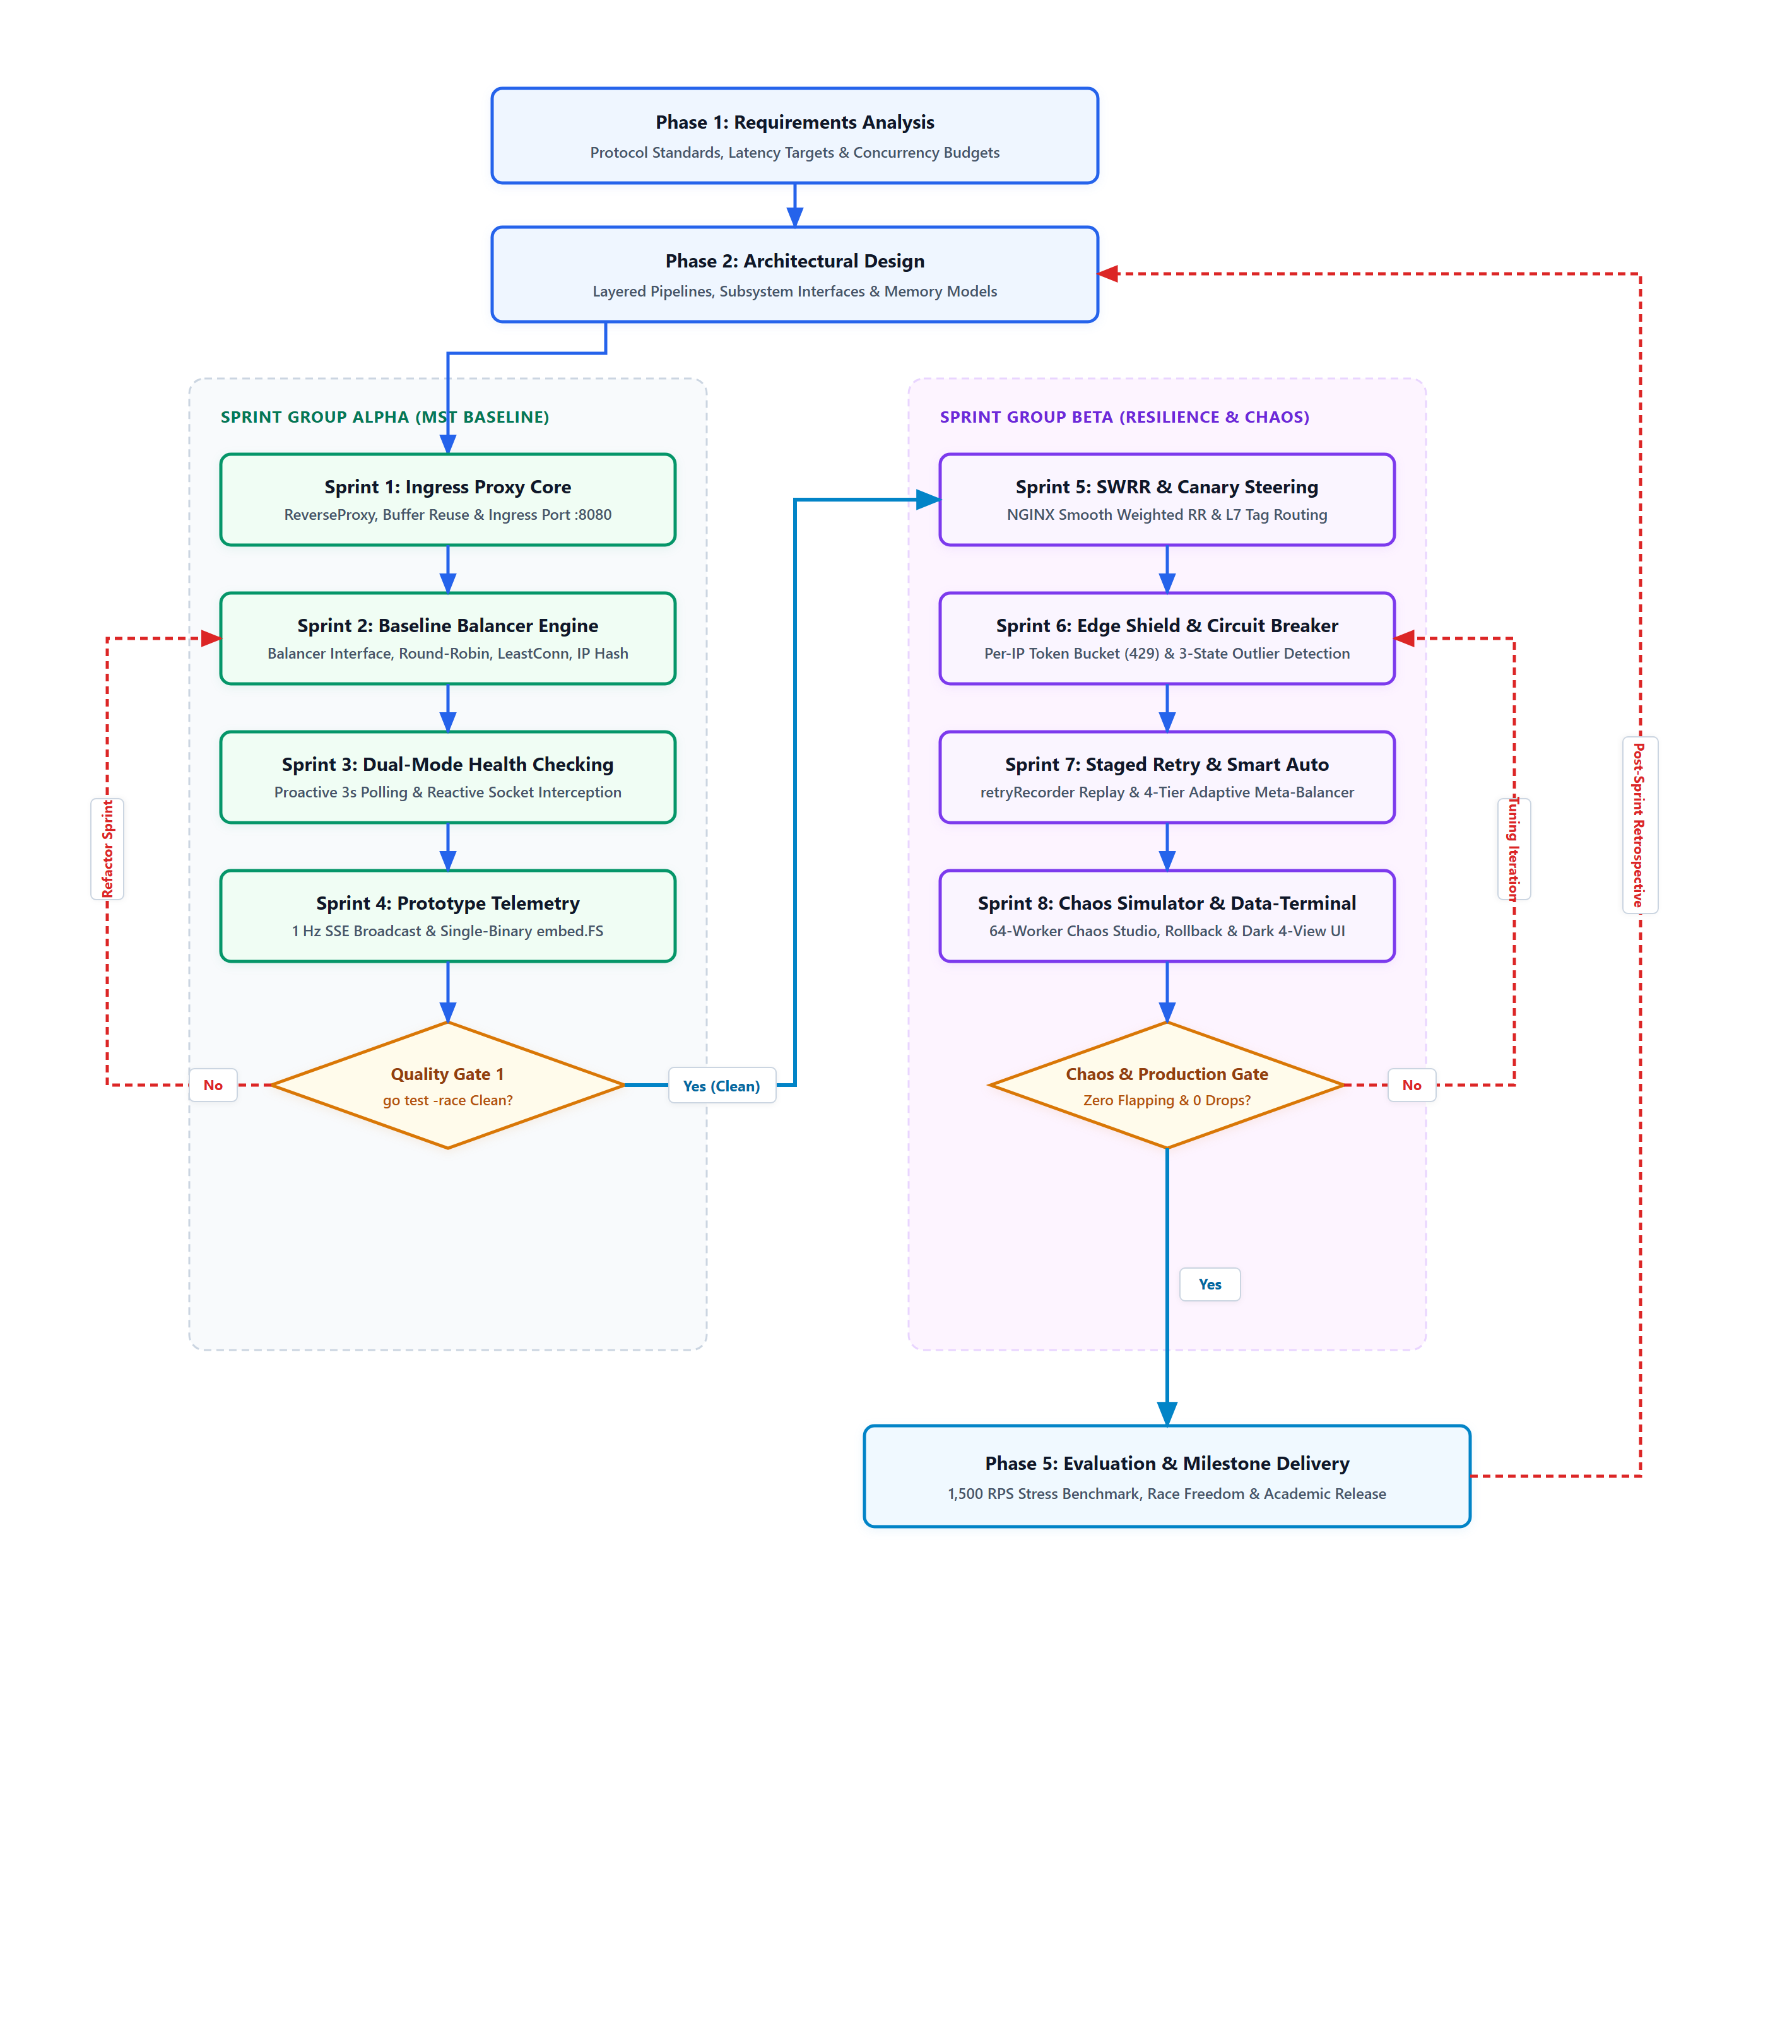
\includegraphics[width=0.96\textwidth]{images/figure_2_1_sdlc.png}
\caption{8-Sprint Agile Incremental Iterative SDLC model applied throughout the NexusLB project.}
\label{fig:sdlc_diagram}
\end{figure}

\section{System Architecture and Requirements Specification}

To guarantee architectural integrity and establish verification criteria, NexusLB was designed against 12 formal Functional Requirements (FR) and 8 Non-Functional Requirements (NFR).

\subsection{Functional Requirements (FR)}
\begin{itemize}
  \item \textbf{FR1 (Dynamic Multi-Algorithm Ingress):} The system shall support five routing algorithms (Round-Robin, Least Connections, Deterministic IP Hash, Smooth Weighted Round-Robin, and Smart Auto Adaptive) hot-swappable at runtime without process restarts.
  \item \textbf{FR2 (Smooth Weighted Balancing):} The system shall implement NGINX's smooth weighted round-robin algorithm, dynamically decrementing and smoothly restoring effective weights upon node failure and recovery.
  \item \textbf{FR3 (Smart Auto Meta-Balancing):} The system shall monitor cluster telemetry and autonomously switch routing algorithms using a 4-tier priority cascade (Queue Skew $\rightarrow$ Weight Variance $\rightarrow$ Session Sticky $\rightarrow$ Round-Robin).
  \item \textbf{FR4 (Hysteresis & Flapping Mitigation):} The adaptive engine shall enforce an asymmetric cooldown timer ($T_{dwell} \ge 4.0\,\text{s}$) to prevent oscillation between algorithms under fluctuating workloads.
  \item \textbf{FR5 (Explainability & Transition Auditing):} The adaptive engine shall generate real-time explainability snapshots detailing why an algorithm was selected and record timestamped transition logs.
  \item \textbf{FR6 (Ingress Edge Shield Rate Limiting):} The system shall enforce per-IP Token Bucket rate limiting, returning standardized $HTTP~429~Too~Many~Requests$ with $Retry-After$ headers when burst limits are exceeded.
  \item \textbf{FR7 (Memory Sweeper for Rate Limiter):} The rate limiter shall execute a background garbage collection worker every 60 seconds to evict inactive client IP buckets and prevent memory leaks.
  \item \textbf{FR8 (Three-State Circuit Breaking):} The proxy shall maintain a circuit breaker for each backend with \texttt{Closed}, \texttt{Open}, and \texttt{Half-Open} states, tripping to \texttt{Open} after 5 consecutive failures.
  \item \textbf{FR9 (Transparent Staged Retries):} In-flight requests encountering network resets or 5xx server errors shall be transparently retried against alternate healthy nodes using a staged body buffer (\texttt{retryRecorder}).
  \item \textbf{FR10 (Layer 7 Canary Traffic Steering):} Ingress requests matching canary criteria (header \texttt{X-Canary: true}, cookie, or query parameter) shall be deterministically isolated to designated canary backends.
  \item \textbf{FR11 (Autonomous Chaos Simulator):} The system shall provide an embedded 64-worker traffic simulation studio capable of executing 6 configurable attack waves (DoS, Botnet, Outage, Latency, Canary, Bursts).
  \item \textbf{FR12 (Atomic Reversible Rollback):} The simulation engine shall capture a baseline snapshot (\texttt{chaosBackup}) prior to wave execution and provide atomic restoration to pristine cluster states.
\end{itemize}

\subsection{Non-Functional Requirements (NFR)}
\begin{itemize}
  \item \textbf{NFR1 (Sub-Millisecond Routing Latency):} Algorithmic decision overhead across the ingress hot-path shall not exceed $0.5\,\text{ms}$ under baseline operating conditions.
  \item \textbf{NFR2 (High Throughput & Concurrency):} The gateway shall sustain a minimum of $1,500$ requests per second on consumer-grade quad-core hardware with minimal CPU degradation.
  \item \textbf{NFR3 (Zero-Downtime Hot Swapping):} Swapping balancing strategies or adjusting node weights via management APIs shall complete with zero dropped client connections.
  \item \textbf{NFR4 (Concurrency Safety & Race Freedom):} All shared memory structures must be synchronized via atomic operations (\texttt{sync/atomic}) or reader-writer mutexes (\texttt{sync.RWMutex}), verified clean under Go's race detector.
  \item \textbf{NFR5 (Bounded Memory Footprint):} The executable and in-memory ring buffers shall maintain a stable resident set size (RSS) under 64\,MB during continuous 1,500 RPS workloads.
  \item \textbf{NFR6 (Single-Binary Self-Contained Deployment):} The gateway, reverse proxy, simulator engine, and web dashboard assets must compile into a single static binary with zero external runtime dependencies.
  \item \textbf{NFR7 (Telemetry Latency & Zero DOM Thrashing):} Real-time metrics streaming over SSE shall push at exactly 1\,Hz with client-side ring buffers capped at 24 points to avoid browser memory leaks.
  \item \textbf{NFR8 (Fault Isolation & Self-Healing Time):} Sudden upstream node crashes must be isolated within $0\,\text{ms}$ reactively, and restored nodes smoothly reintegrated within $\le 3.0\,\text{seconds}$.
\end{itemize}

\subsection{Use Case Analysis}

Figure~\ref{fig:usecase_diagram} depicts the UML Use Case Diagram for NexusLB, illustrating the system boundary, external actors (Client Consumer, Upstream Node, and DevOps Administrator), and 15 functional associations.

\begin{figure}[H]
\centering
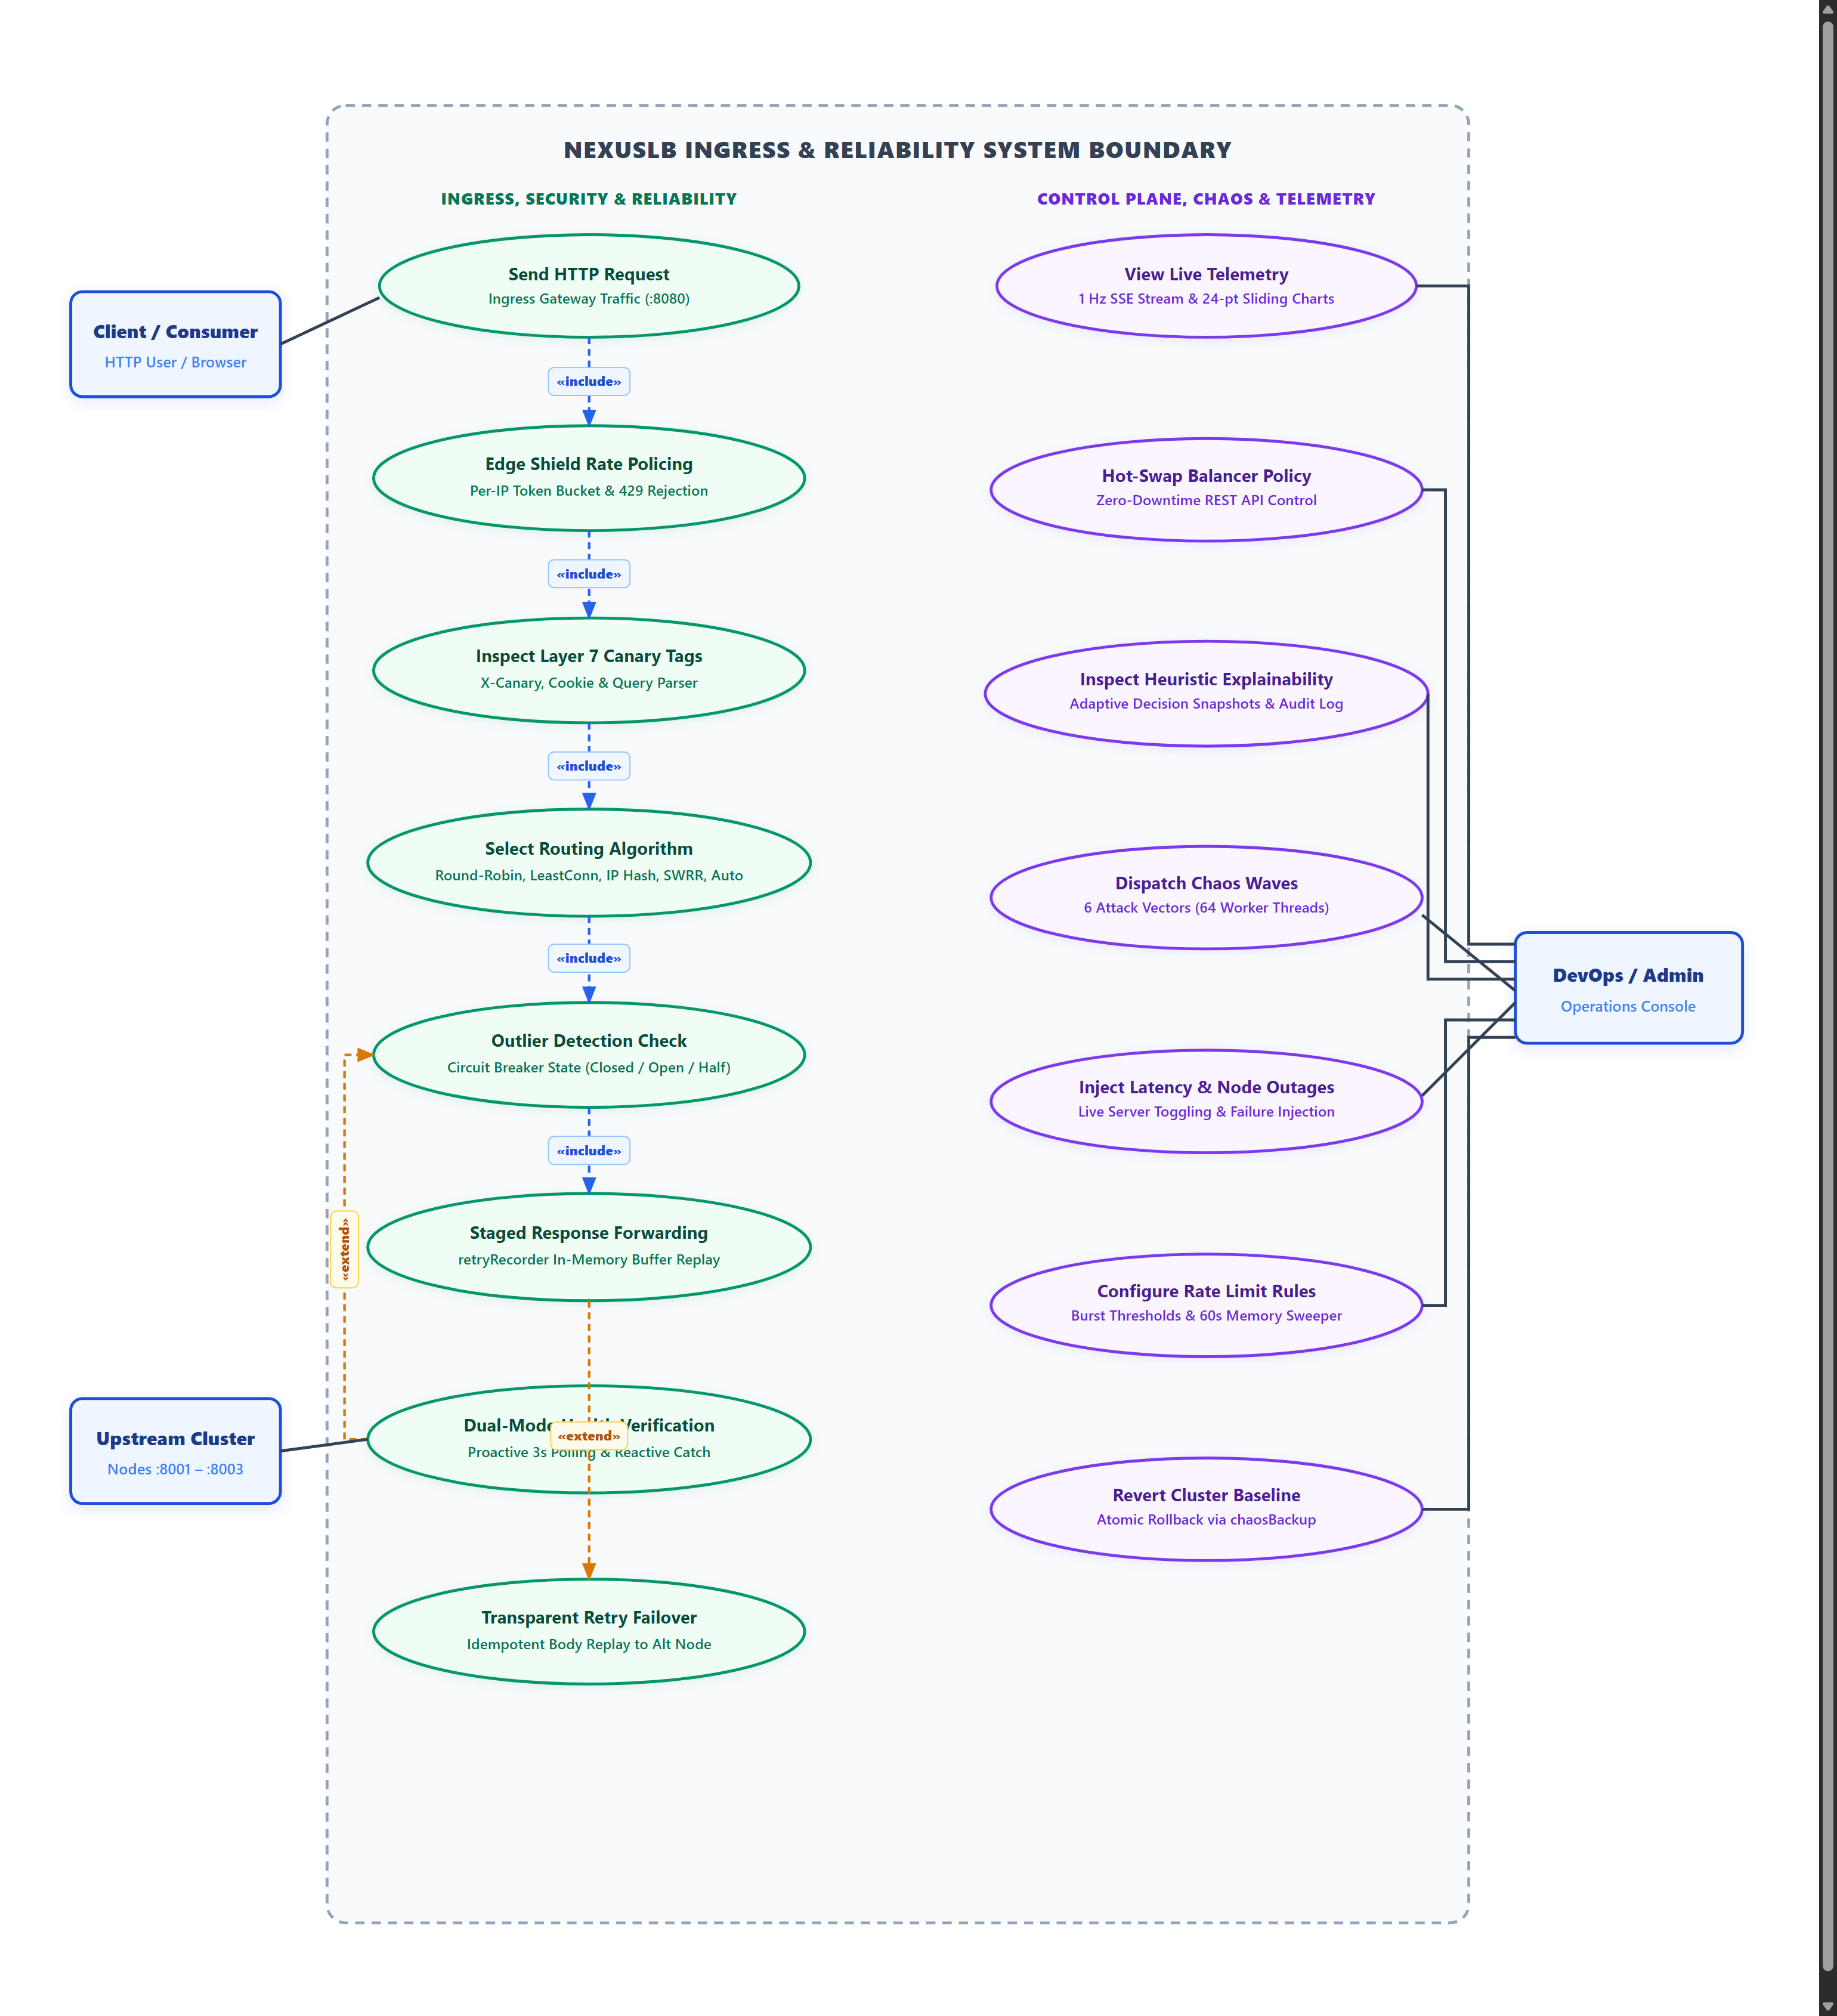
\includegraphics[width=0.96\textwidth]{images/figure_2_2_usecase.png}
\caption{Expanded UML Use Case Diagram illustrating actor roles, system boundary, and 15 functional associations.}
\label{fig:usecase_diagram}
\end{figure}

\subsection{High-Level Layered UML Architecture}

Figure~\ref{fig:uml_arch} illustrates the high-level layered component architecture of NexusLB. Requests pass vertically down the ingress pipeline through the Edge Shield, Canary Classifier, Strategy Manager, and Circuit Breakers before reaching the backend servers, while telemetry and simulation planes interact asynchronously.

\begin{figure}[H]
\centering
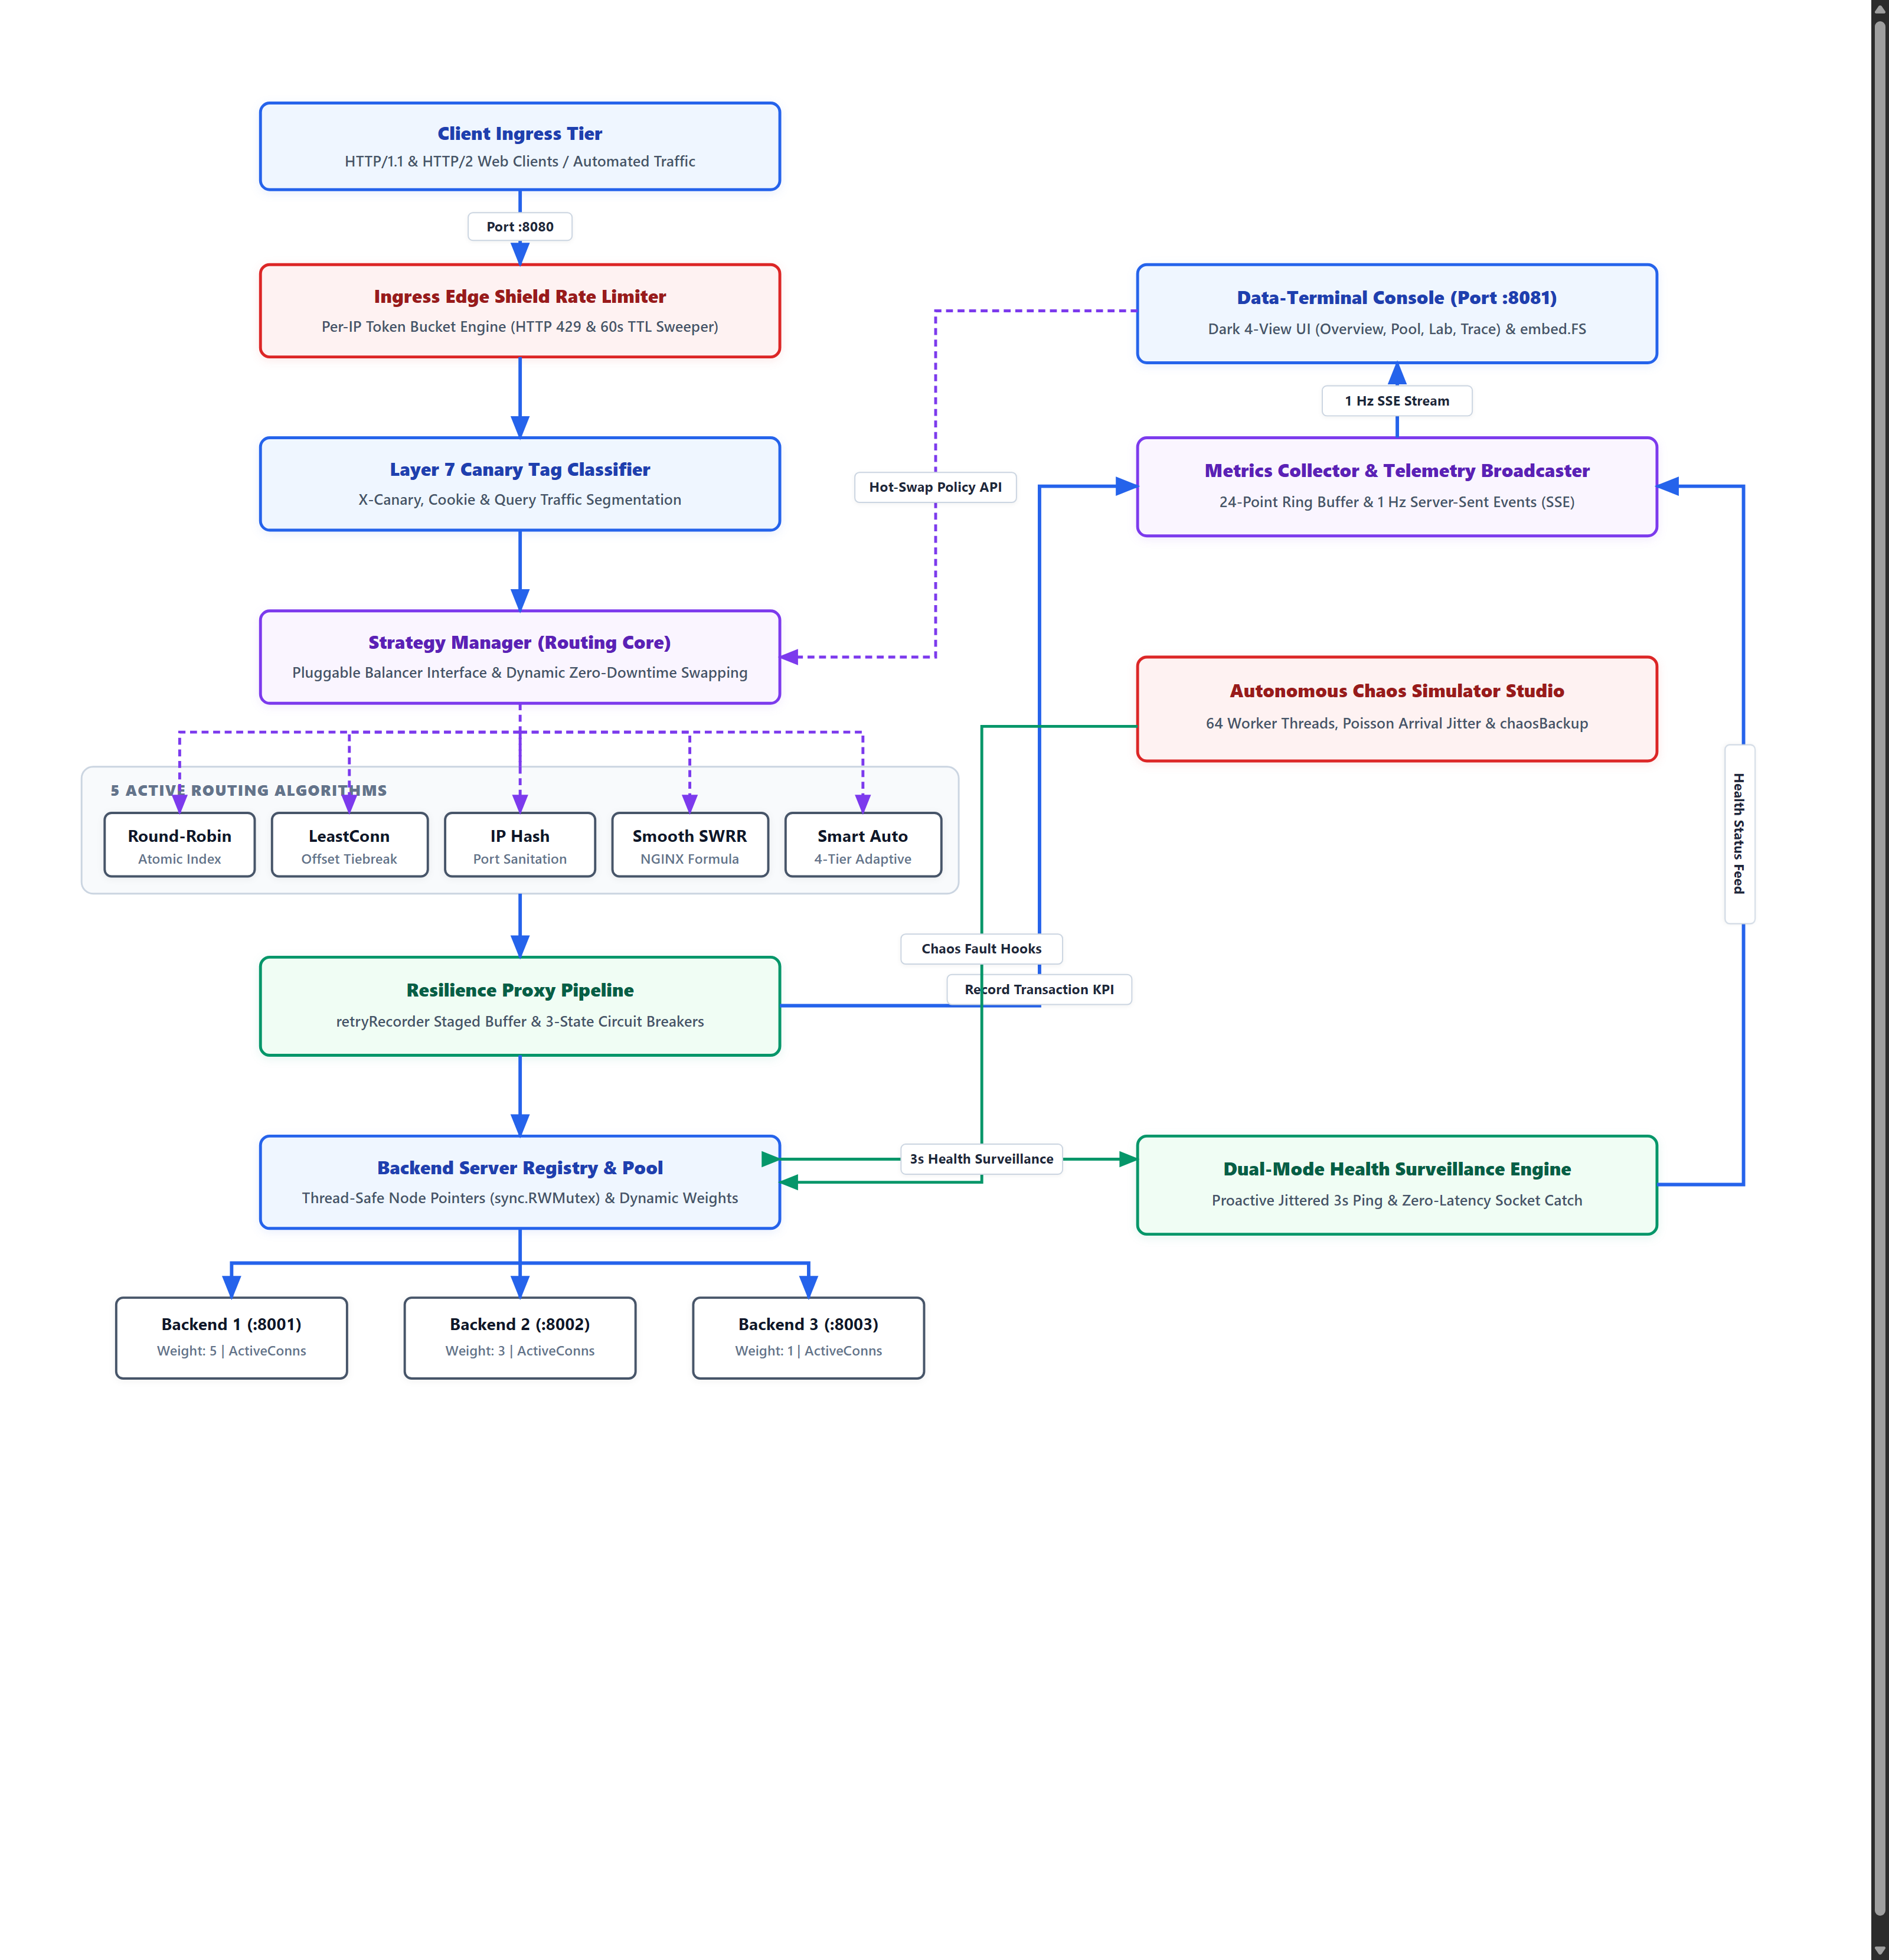
\includegraphics[width=0.96\textwidth]{images/figure_2_3_arch.png}
\caption{Layered High-Level UML Architecture of NexusLB showing component pipelines and interaction channels.}
\label{fig:uml_arch}
\end{figure}

\subsection{Physical Component and Deployment Topology}

Figure~\ref{fig:deploy_diagram} shows the physical deployment topology of NexusLB running on a host environment. The gateway exposes port \texttt{:8080} for ingress traffic, port \texttt{:8081} for the management console and SSE stream, and interfaces with the simulated backend pool on ports \texttt{:8001}, \texttt{:8002}, and \texttt{:8003}.

\begin{figure}[H]
\centering
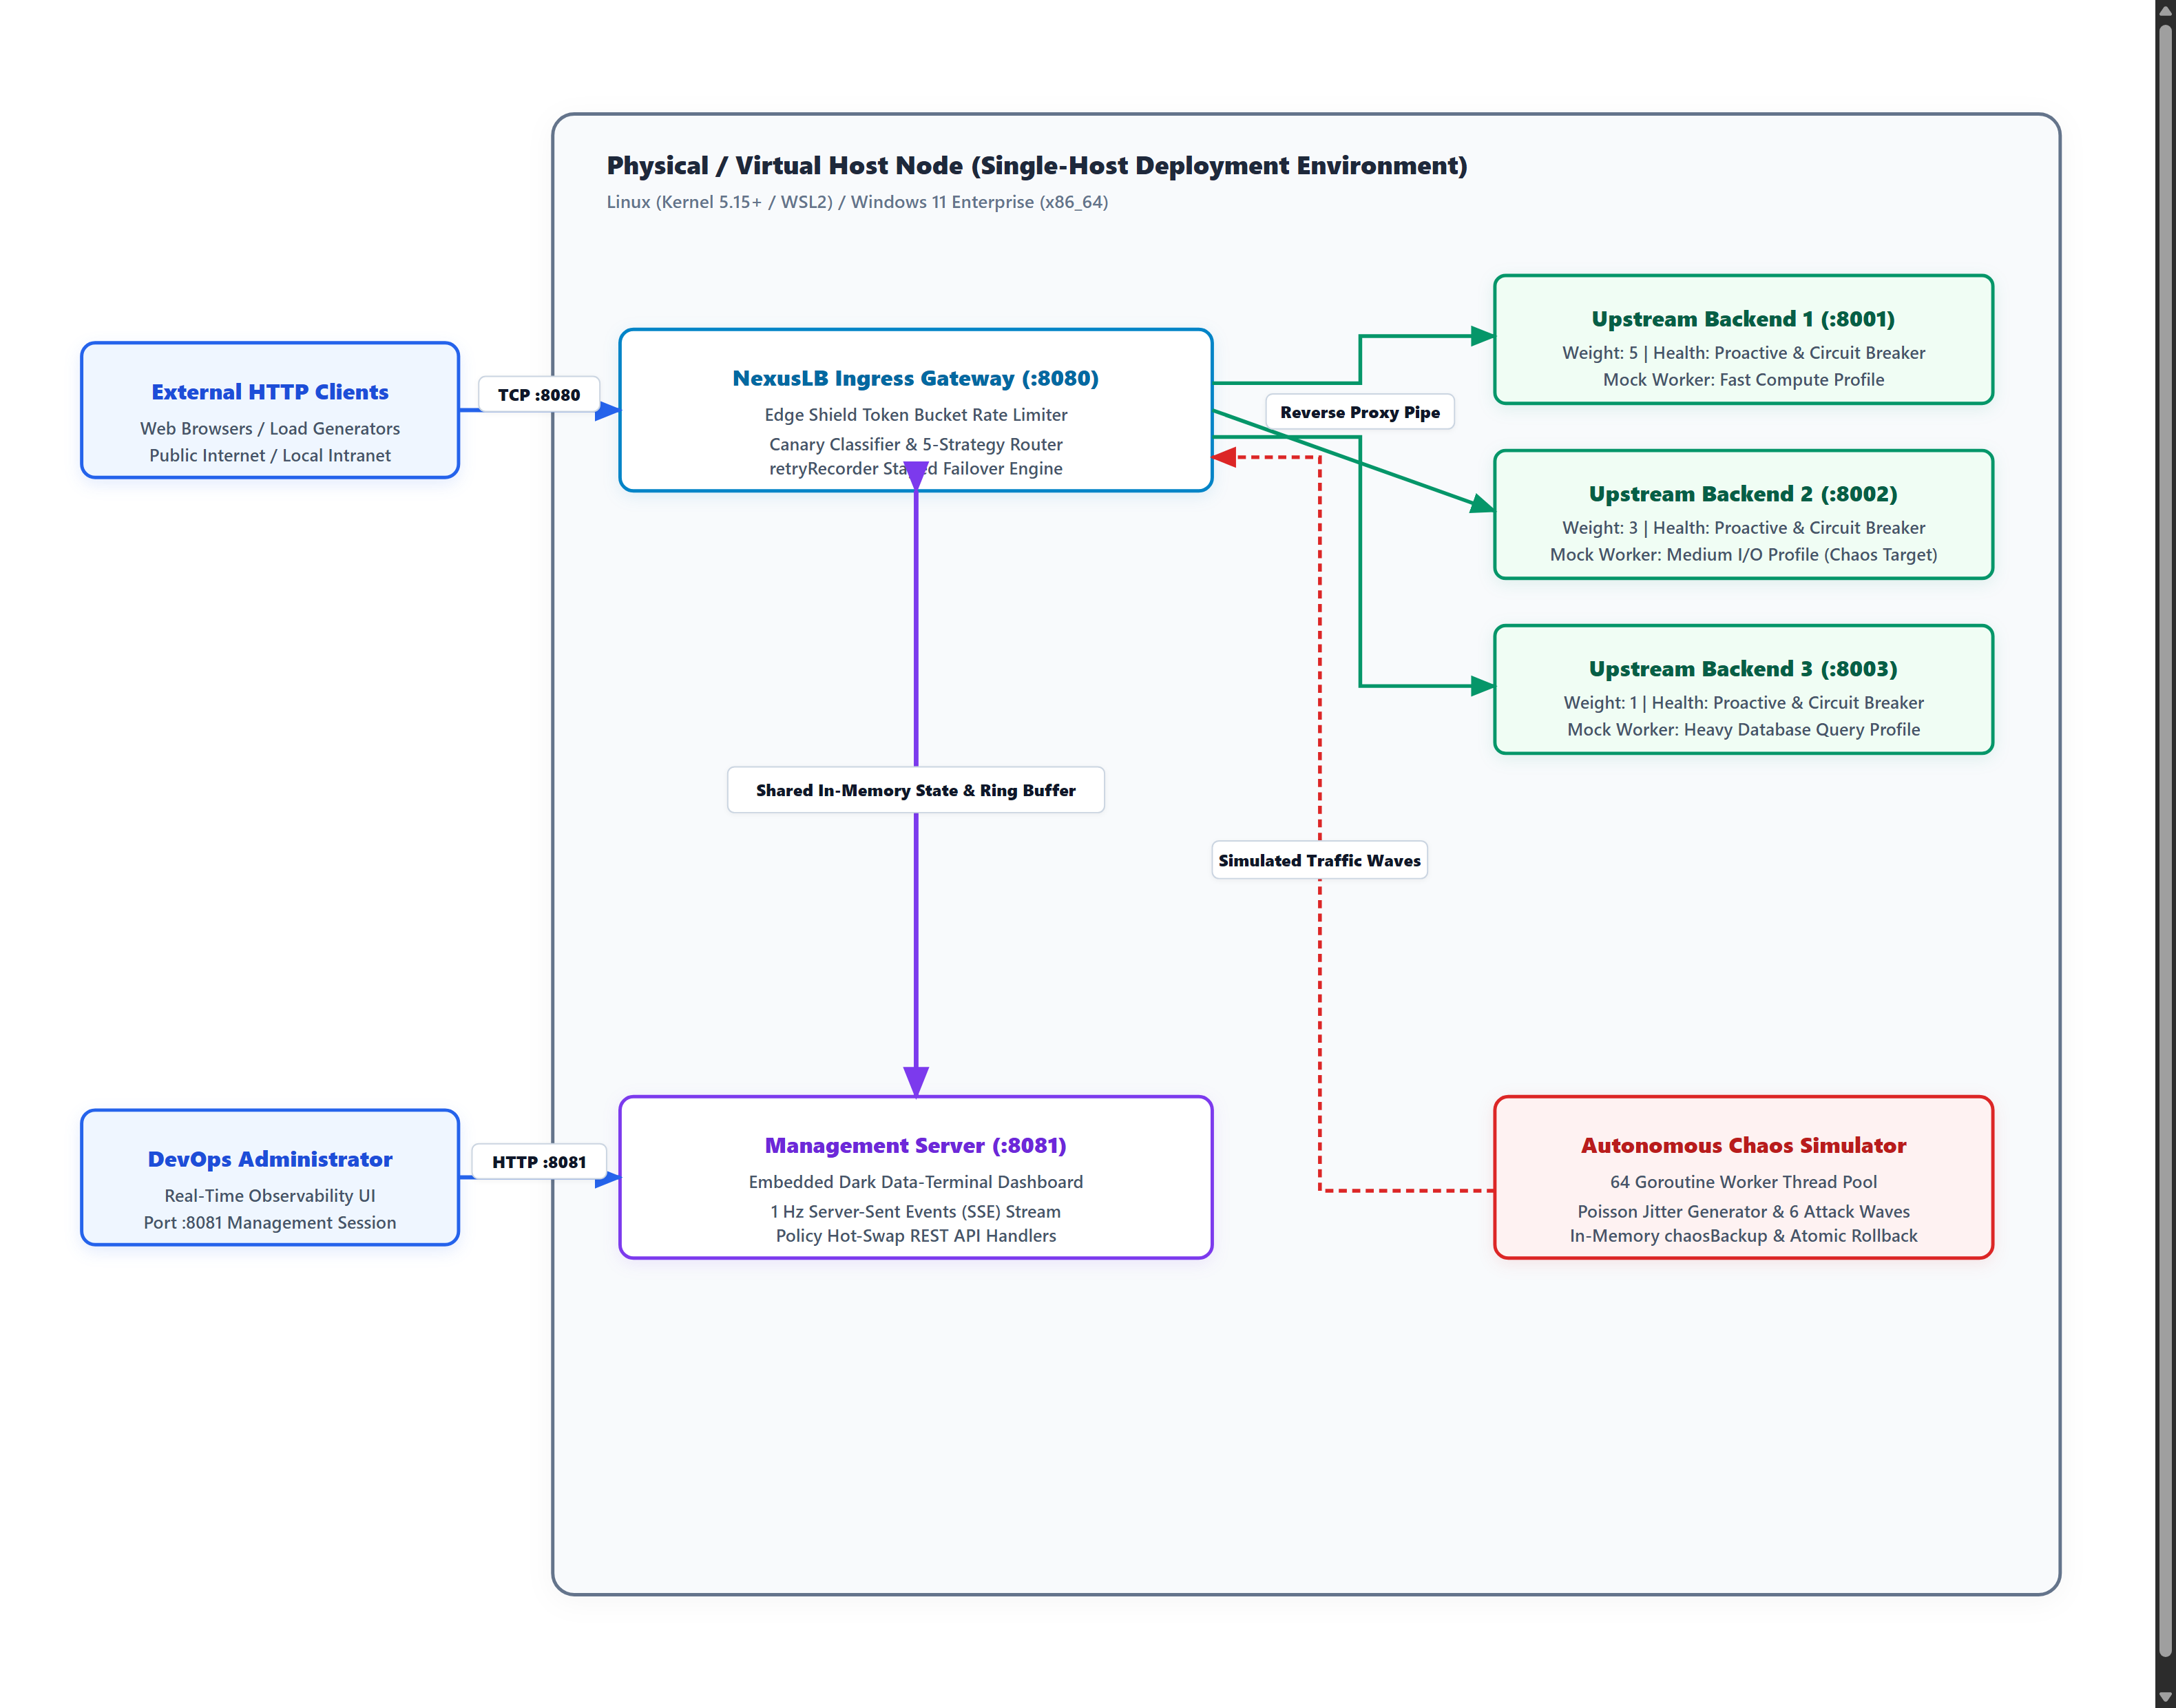
\includegraphics[width=0.96\textwidth]{images/figure_2_4_deploy.png}
\caption{Component and physical deployment topology of NexusLB on a single host runtime.}
\label{fig:deploy_diagram}
\end{figure}



\subsection{Data Flow Modeling (DFD Level 0 and Level 1)}

To document the flow of information through the system, Figure~\ref{fig:dfd_diagram} presents the structured Data Flow Diagram partitioned into Level 0 (Context) and Level 1 (Functional Decomposition).

\begin{figure}[H]
\centering
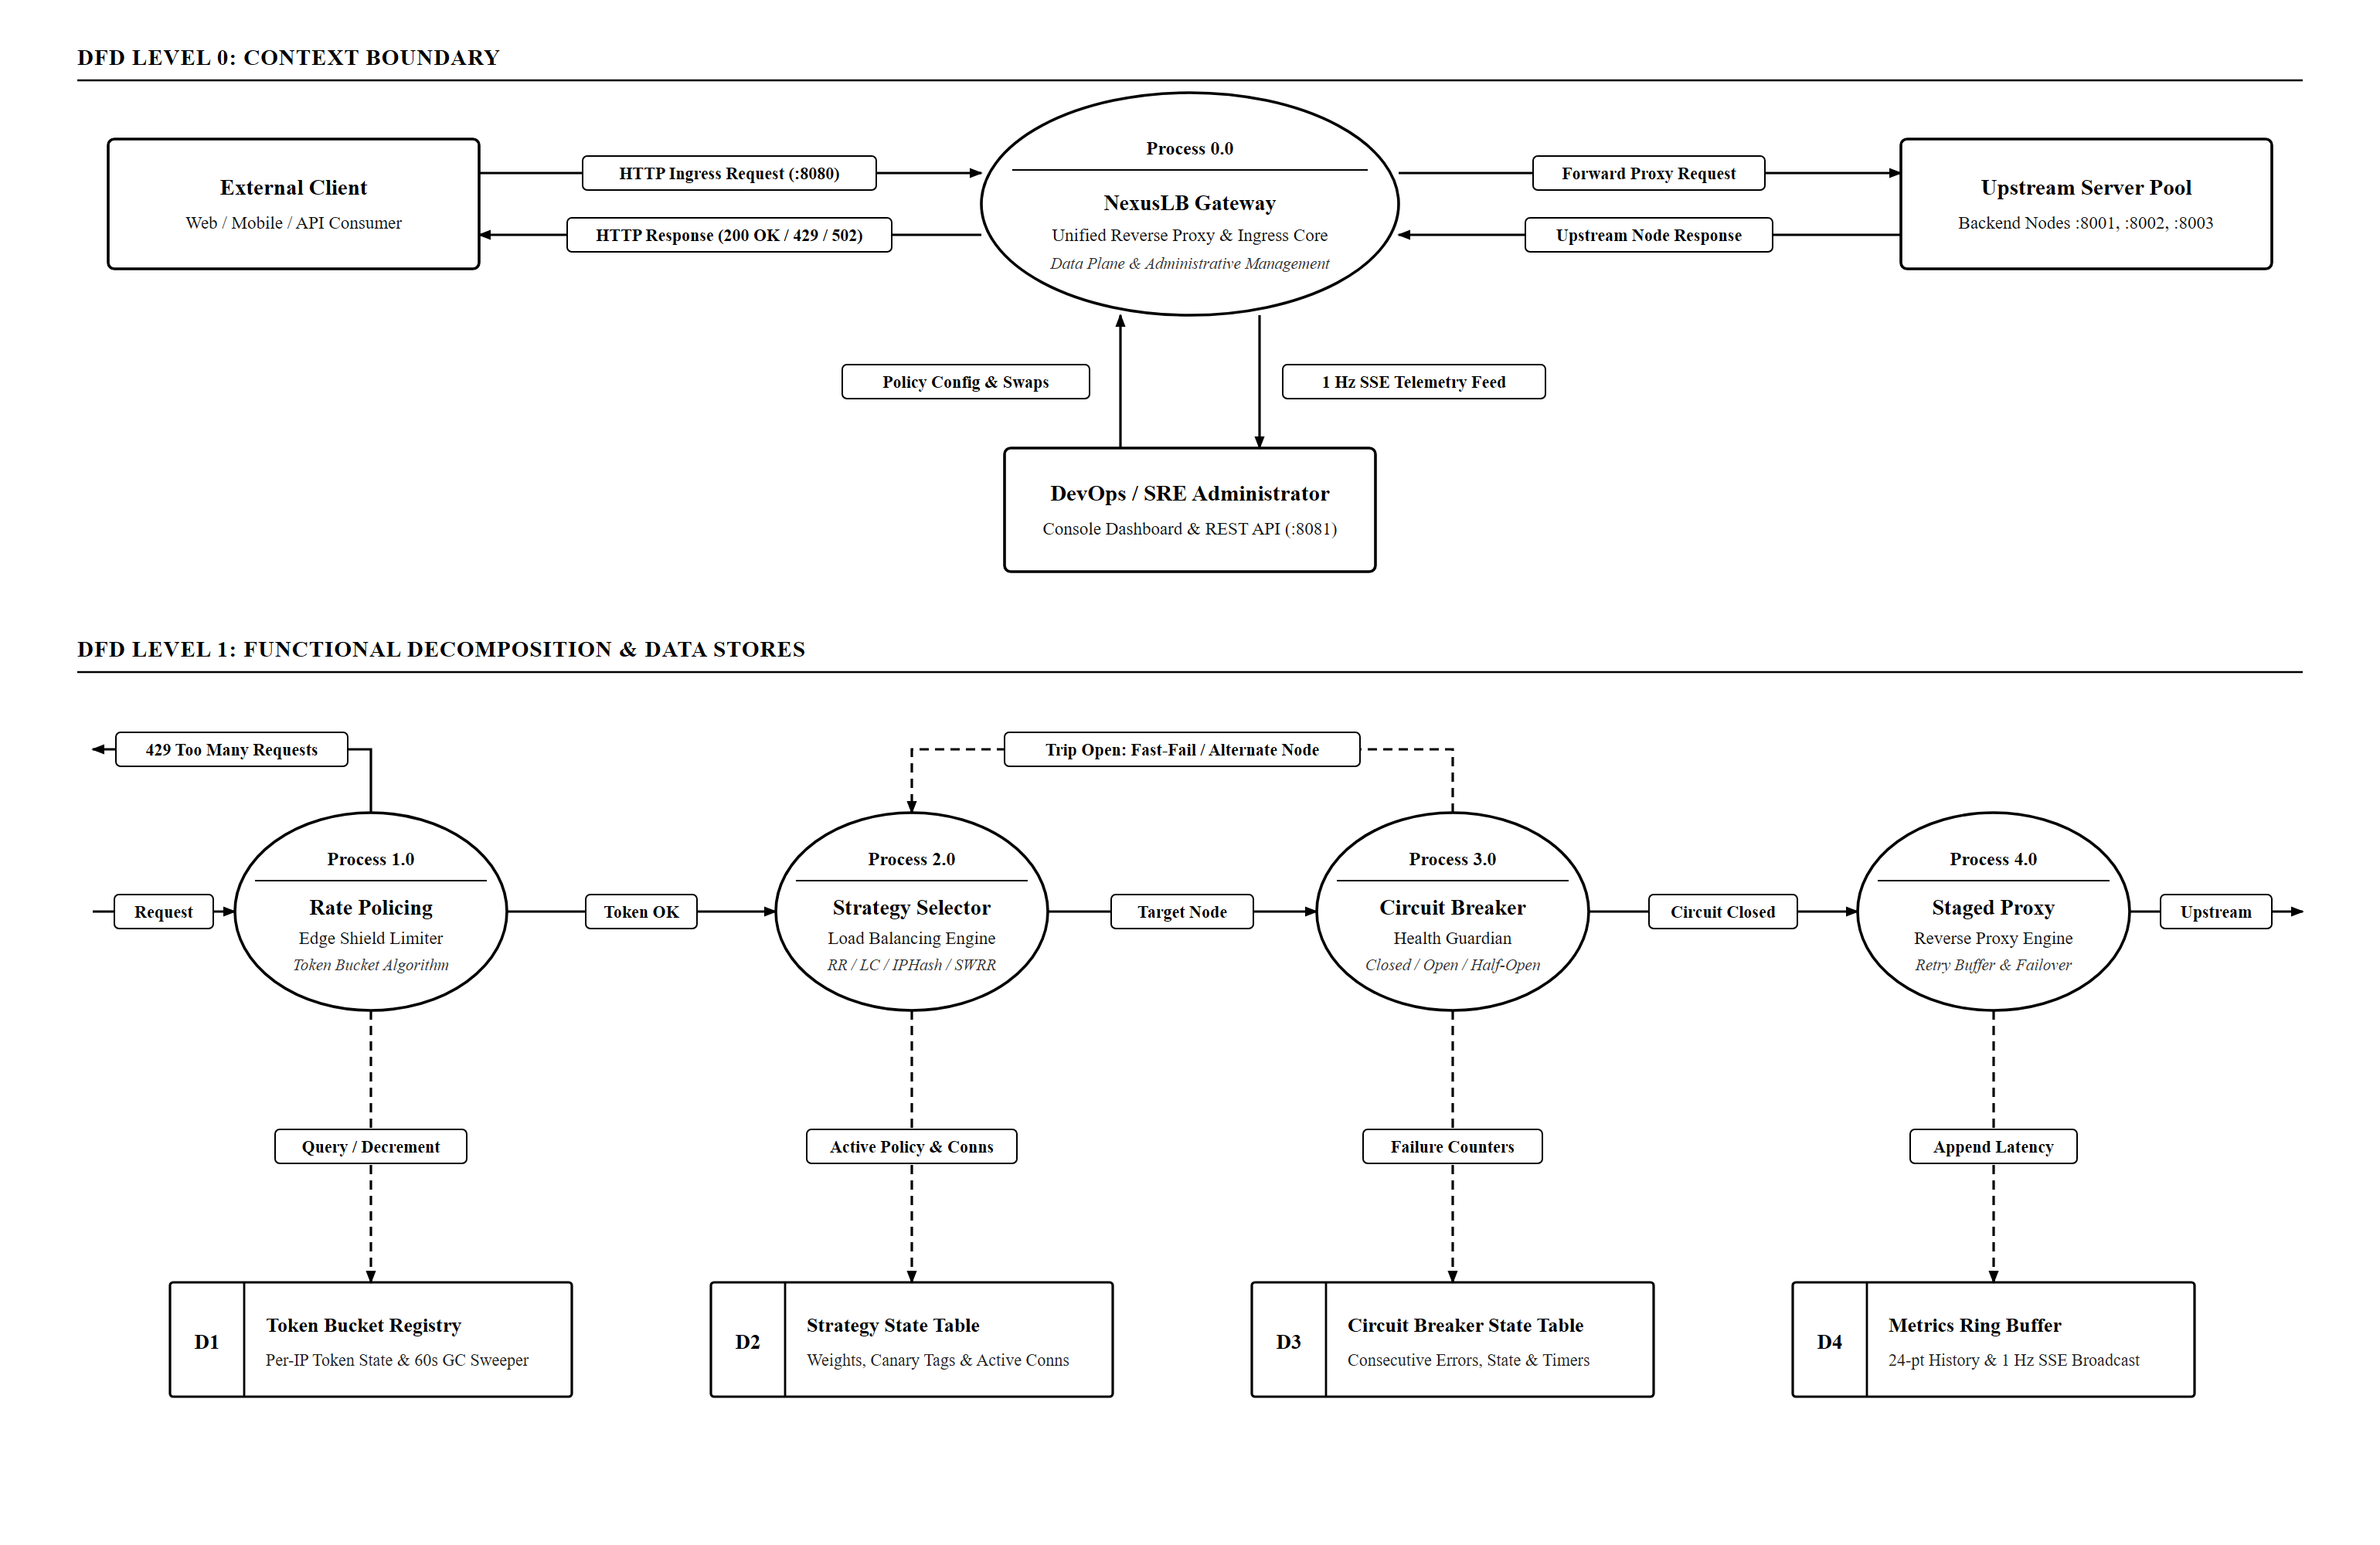
\includegraphics[width=0.96\textwidth]{images/figure_2_5_dfd.png}
\caption{Data Flow Diagrams (Level 0 Context and Level 1 Functional Decomposition) of NexusLB.}
\label{fig:dfd_diagram}
\end{figure}

\section{Detailed Design and Implementation}

\subsection{Object-Oriented Design and Data Structures}

Figure~\ref{fig:class_diagram} presents the detailed UML Class Diagram illustrating Go data structures, interfaces, and associations across the five balancing strategies, rate limiter, circuit breaker, and chaos simulator.

\begin{figure}[H]
\centering
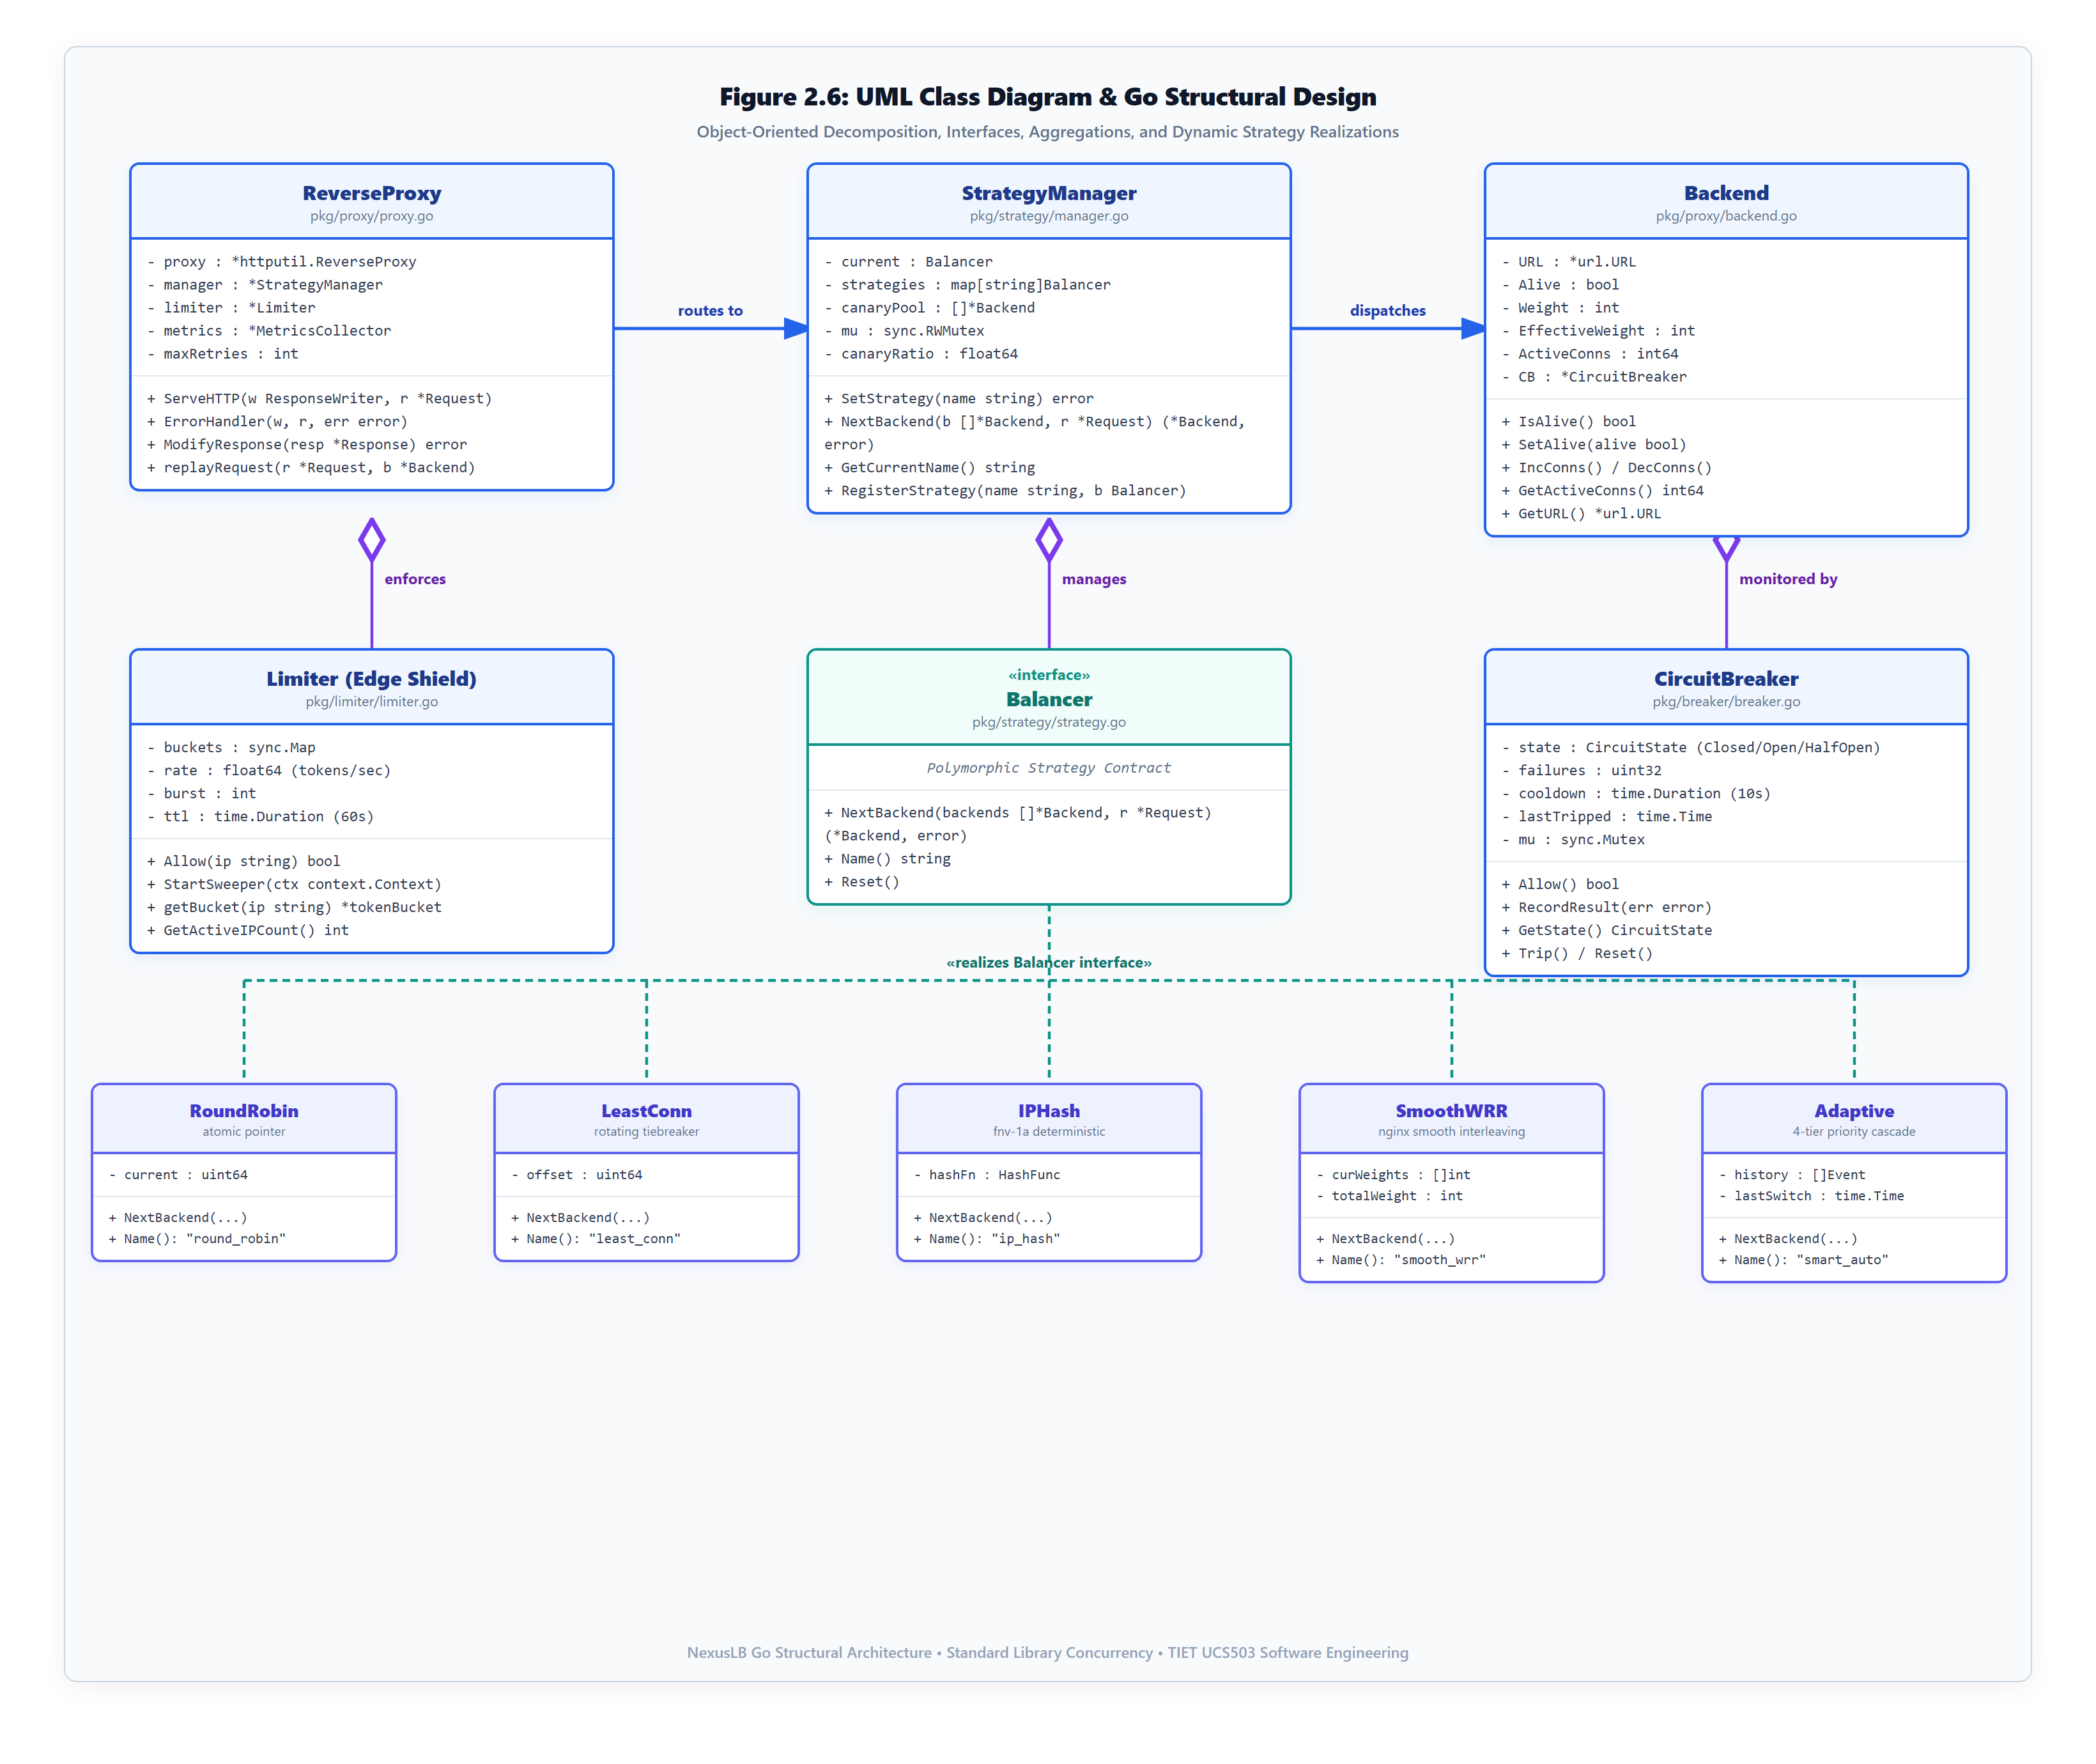
\includegraphics[width=0.96\textwidth]{images/figure_2_6_class.png}
\caption{UML Class Diagram illustrating structural relationships, interfaces, and methods in NexusLB.}
\label{fig:class_diagram}
\end{figure}

\subsection{Core Request Workflow and Activity Model}

Figure~\ref{fig:activity_diagram} details the execution path of an incoming HTTP request through rate limiting, canary routing, algorithm evaluation, circuit breaker checking, staged retry recording, and metrics dispatch.

\begin{figure}[H]
\centering
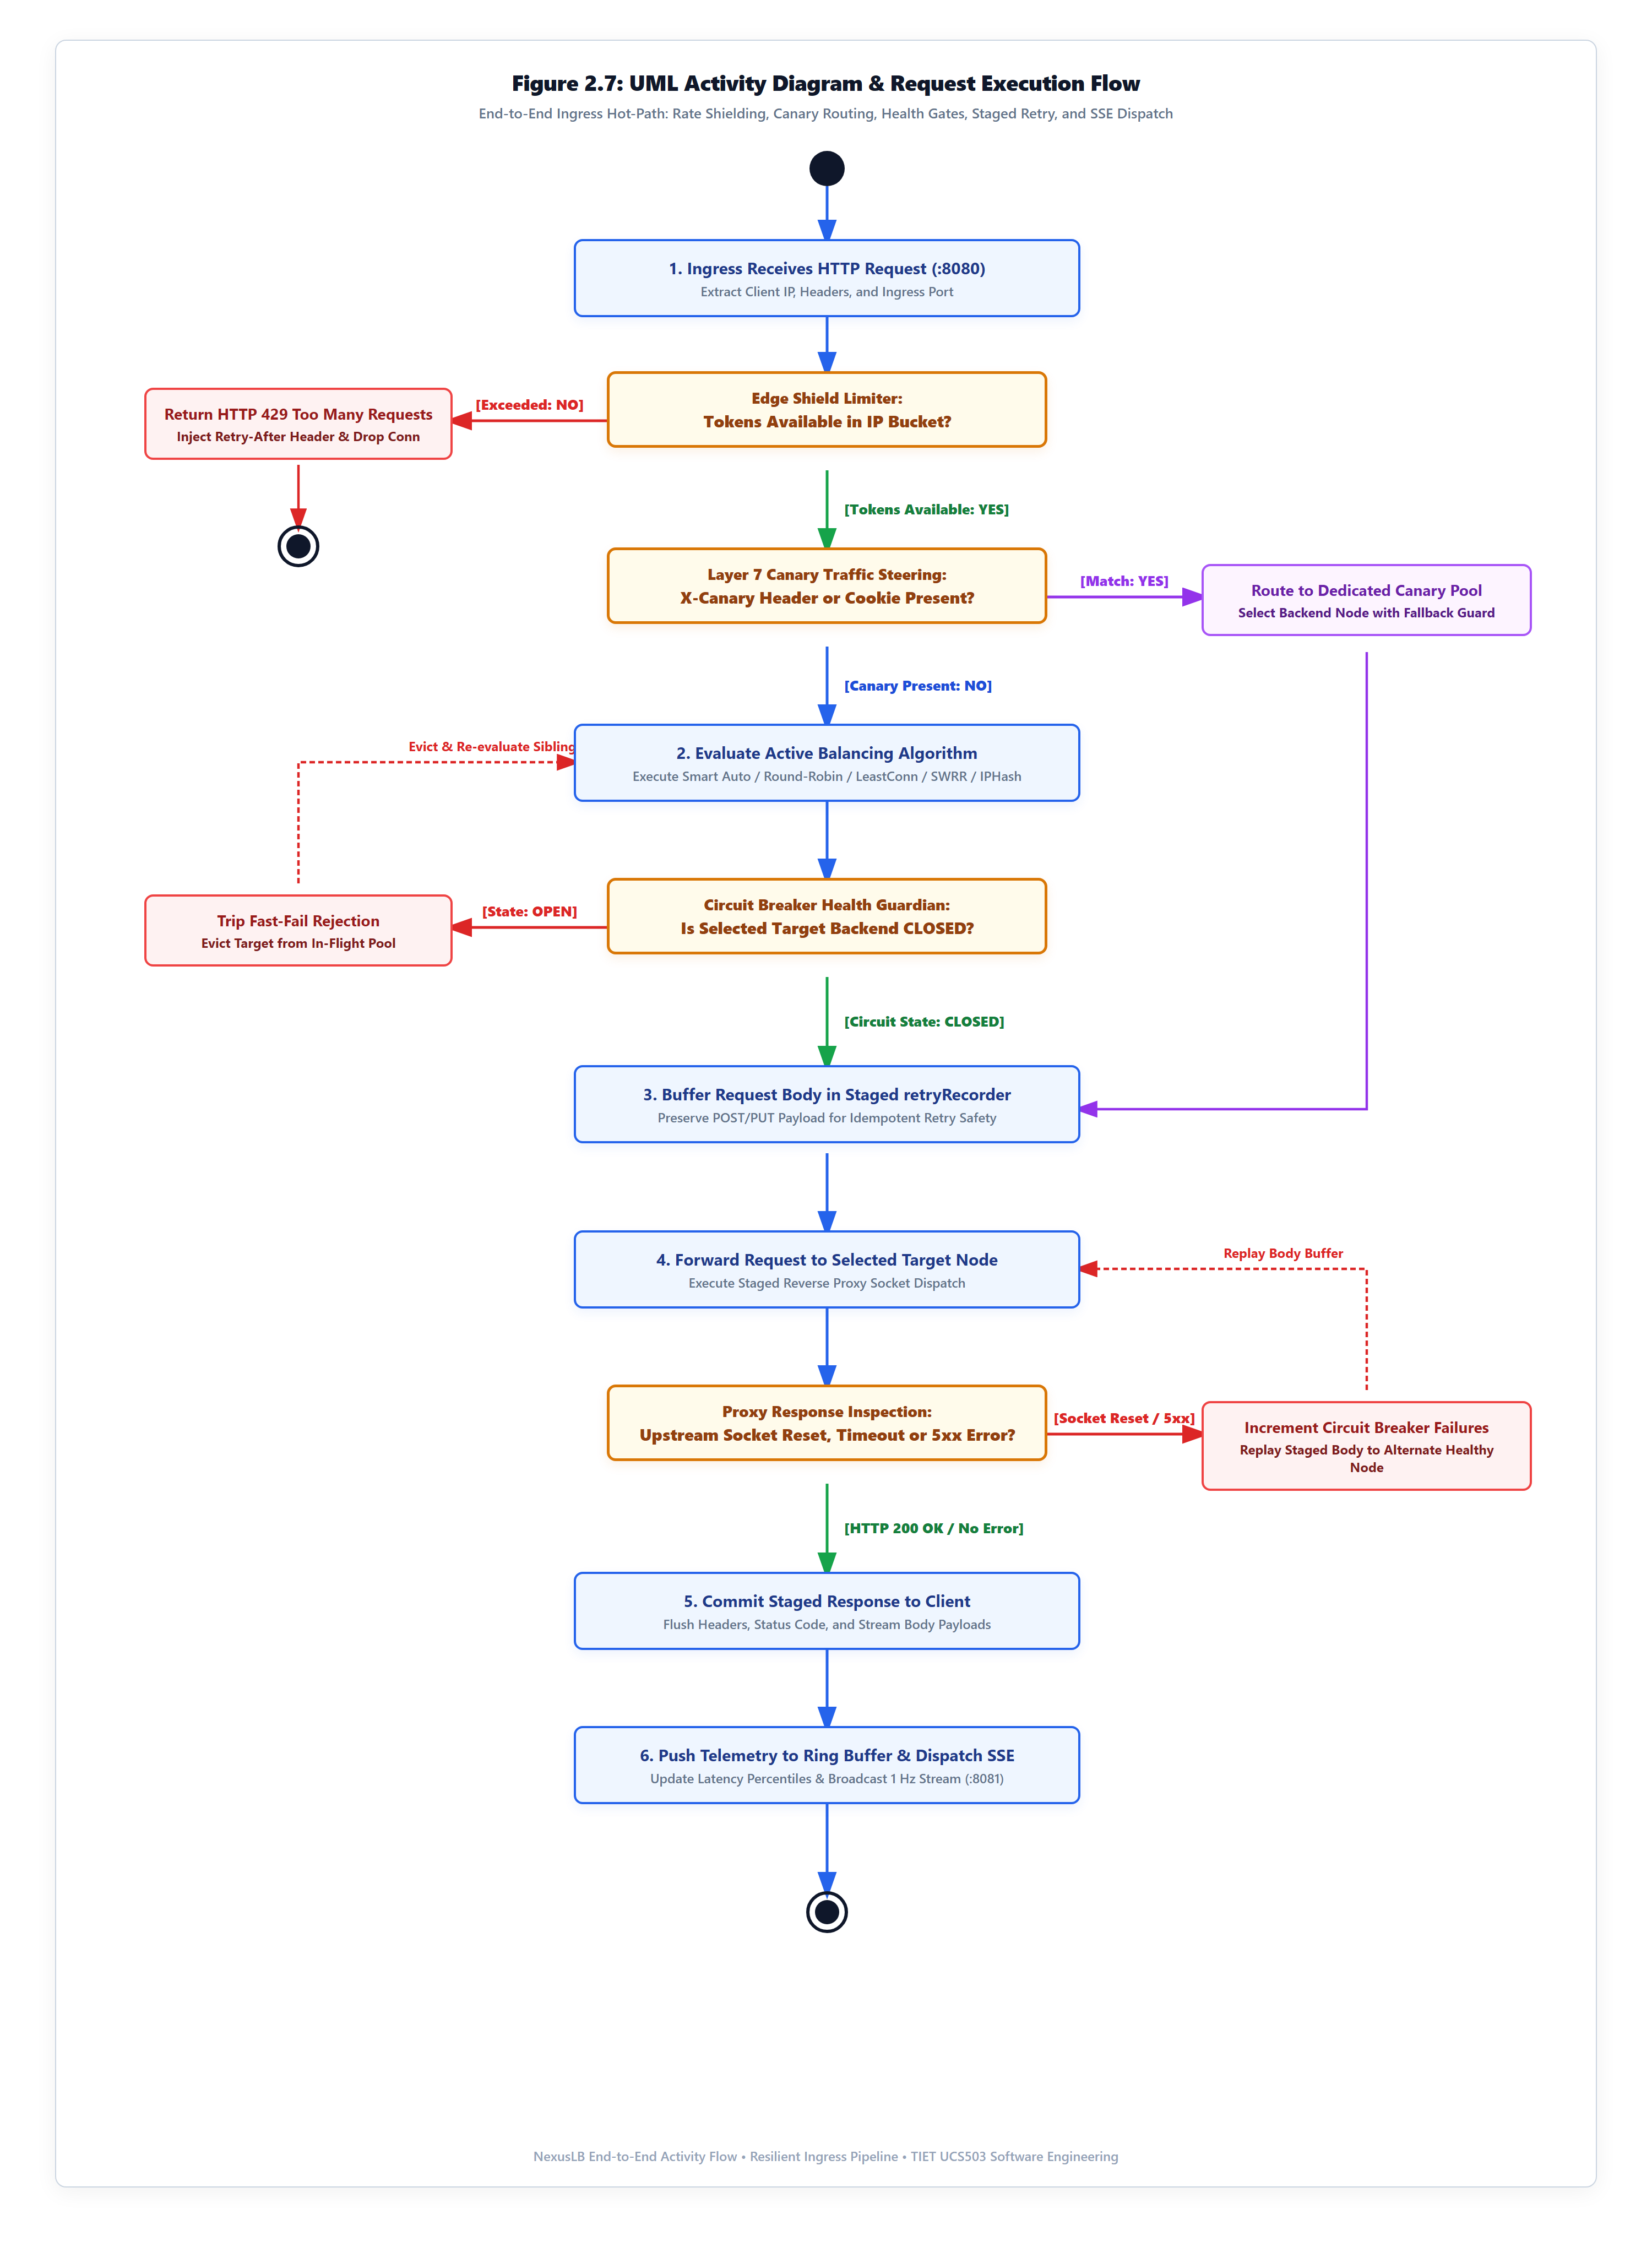
\includegraphics[width=0.96\textwidth]{images/figure_2_7_activity.png}
\caption{UML Activity Diagram detailing the end-to-end request lifecycle through NexusLB.}
\label{fig:activity_diagram}
\end{figure}

\subsection{Load Balancing Strategies}

NexusLB decouples policy from routing mechanics via the Strategy design pattern~\cite{gamma1994} and the unified \texttt{Balancer} interface:
\begin{lstlisting}[language=Go, basicstyle=\ttfamily\footnotesize, frame=single, breaklines=true]
type Balancer interface {
    NextBackend(
        backends []*backend.Backend,
        r *http.Request,
    ) (*backend.Backend, error)
    Name() string
}
\end{lstlisting}

\textbf{Round-Robin with Atomic Indexing:} For homogeneous clusters, Round-Robin provides mathematically uniform request distribution without lock contention using 64-bit atomic pointer arithmetic:
\begin{equation}
i = (\text{atomic.AddUint64}(\&rr.current, 1) - 1) \pmod n
\end{equation}

\textbf{Least Connections with Rotating Offset:} Under heterogeneous request costs, Least Connections inspects active connection counts. An atomic offset tiebreaker guarantees uniform distribution across idle instances:
\begin{equation}
\text{start\_index} = \text{atomic.AddUint64}(\&lc.offset, 1) \pmod n
\end{equation}

\textbf{Deterministic IP Hash with TCP Port Sanitation:} Standardizes loopback formats, strips ephemeral client TCP ports, and computes deterministic routing:
\begin{equation}
h = \text{fnv32a}(\text{cleanIP}) \pmod n
\end{equation}

\textbf{Smooth Weighted Round-Robin (SWRR - NGINX Algorithm):} When nodes possess heterogeneous compute capacities, NexusLB implements NGINX's smooth weighted round-robin algorithm~\cite{nginx_swrr}:
\begin{align}
CW_i &\leftarrow CW_i + EW_i \\
b^* &= \arg\max_{i} (CW_i) \\
CW_{b^*} &\leftarrow CW_{b^*} - \sum_{j=1}^{n} EW_j
\end{align}
Effective weights $EW_i$ decay dynamically upon failures and smoothly ramp back upon verified health recovery.

\subsection{Smart Auto Adaptive Meta-Balancing}

The \textbf{Smart Auto} (\texttt{adaptive}) meta-balancer continuously inspects telemetry signals across a 4-tier decision cascade:
\begin{enumerate}
  \item \textbf{Tier 1 (Queue Imbalance):} $\Delta = \max(Conns) - \min(Conns) > 15 \implies$ \textbf{Least Connections}.
  \item \textbf{Tier 2 (Capacity Skew):} $W_{\max}/W_{\min} \ge 1.5 \implies$ \textbf{Smooth Weighted RR}.
  \item \textbf{Tier 3 (Session Stickiness):} Session cookies or auth headers $\implies$ \textbf{IP Hash}.
  \item \textbf{Tier 4 (Homogeneous Baseline):} Default fallback $\implies$ \textbf{Round-Robin}.
\end{enumerate}

To prevent rapid oscillation (flapping), an asymmetric hysteresis gate enforces $T_{dwell} \ge 4.0\,\text{s}$ on downward transitions, while emergency escalations ($\Delta > 25$) bypass the cooldown immediately. Every decision emits an \texttt{AdaptiveSnapshot} to the observability console for operator explainability.

Figure~\ref{fig:adaptive_tree} illustrates the priority cascade and hysteresis state machine.

\begin{figure}[H]
\centering
\resizebox{0.95\textwidth}{!}{%
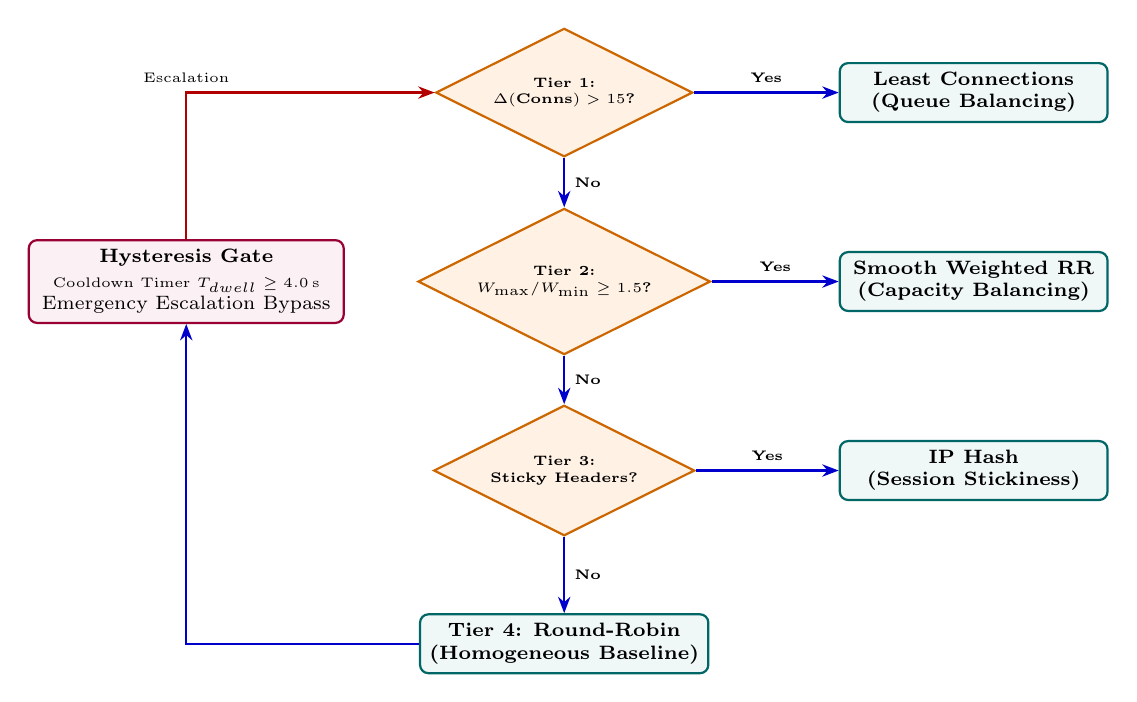
\begin{tikzpicture}[
  font=\scriptsize,
  evalnode/.style={
    diamond,
    aspect=2.0,
    draw=orange!80!black,
    fill=orange!10,
    thick,
    align=center,
    font=\tiny\bfseries
  },
  algonode/.style={
    rectangle,
    rounded corners=3pt,
    draw=teal!80!black,
    fill=teal!6,
    thick,
    minimum width=3.4cm,
    minimum height=0.7cm,
    align=center,
    font=\scriptsize\bfseries
  },
  cooldownnode/.style={
    rectangle,
    rounded corners=3pt,
    draw=purple!80!black,
    fill=purple!6,
    thick,
    minimum width=4.0cm,
    minimum height=0.9cm,
    align=center
  },
  arrow/.style={
    -{Stealth[scale=0.9]},
    thick,
    draw=blue!80!black
  },
  redarrow/.style={
    -{Stealth[scale=0.9]},
    thick,
    draw=red!70!black
  }
]

% Decision Nodes (Vertical Spine)
\node[evalnode] (d1) at (0, 0) {Tier 1:\\$\Delta(\text{Conns}) > 15$?};
\node[evalnode] (d2) at (0, -2.4) {Tier 2:\\$W_{\max}/W_{\min} \ge 1.5$?};
\node[evalnode] (d3) at (0, -4.8) {Tier 3:\\Sticky Headers?};
\node[algonode] (rr) at (0, -7.0) {Tier 4: Round-Robin\\(Homogeneous Baseline)};

% Outcoming Algorithm Nodes (Right)
\node[algonode] (lc) at (5.2, 0) {Least Connections\\(Queue Balancing)};
\node[algonode] (swrr) at (5.2, -2.4) {Smooth Weighted RR\\(Capacity Balancing)};
\node[algonode] (iph) at (5.2, -4.8) {IP Hash\\(Session Stickiness)};

% Cooldown Gate (Left)
\node[cooldownnode] (cd) at (-4.8, -2.4) {\textbf{Hysteresis Gate}\\[1pt]\tiny Cooldown Timer $T_{dwell} \ge 4.0\,\text{s}$\\Emergency Escalation Bypass};

% Flows
\draw[arrow] (d1) -- node[above, font=\tiny\bfseries]{Yes} (lc);
\draw[arrow] (d1) -- node[right, font=\tiny\bfseries]{No} (d2);
\draw[arrow] (d2) -- node[above, font=\tiny\bfseries]{Yes} (swrr);
\draw[arrow] (d2) -- node[right, font=\tiny\bfseries]{No} (d3);
\draw[arrow] (d3) -- node[above, font=\tiny\bfseries]{Yes} (iph);
\draw[arrow] (d3) -- node[right, font=\tiny\bfseries]{No} (rr);

\draw[redarrow] (cd.north) |- node[above, font=\tiny]{Escalation} (d1.west);
\draw[arrow] (rr.west) -| (cd.south);

\end{tikzpicture}%
}
\caption{Adaptive decision priority cascade and asymmetric hysteresis state machine.}
\label{fig:adaptive_tree}
\end{figure}

\subsection{Ingress Edge Shield Rate Limiting}

The inline Edge Shield rate limiter enforces per-IP token bucket policing:
\begin{equation}
\text{tokens} = \min\Big(B, \;\; \text{tokens} + (t_{now} - t_{last}) \times R\Big)
\end{equation}
Exhausted quotas return $HTTP~429~Too~Many~Requests$ with $Retry-After$ headers~\cite{rfc6585}. Buckets reside in a concurrent \texttt{sync.Map}, with an asynchronous background sweeper purging buckets inactive for $\ge 60\,\text{s}$ to safeguard host memory.

\subsection{Three-State Outlier Detection Circuit Breaking}

NexusLB embeds three-state Outlier Detection Circuit Breakers~\cite{nygard2018, fowler2014} in front of each upstream backend. Figure~\ref{fig:cb_fsm} illustrates the state machine:
\begin{itemize}
  \item \textbf{StateClosed:} Normal flow; consecutive failures are tracked. 5 consecutive socket faults trip the breaker to \textbf{StateOpen}.
  \item \textbf{StateOpen:} Upstream traffic is fast-failed in $0.02\,\text{ms}$, preventing thread starvation. A 10-second cooldown timer is initiated.
  \item \textbf{StateHalfOpen:} Exactly one canary probe is permitted. Probe success ($200~OK$) resets the breaker to \textbf{StateClosed}; probe failure returns the breaker to \textbf{StateOpen}.
\end{itemize}

\begin{figure}[H]
\centering
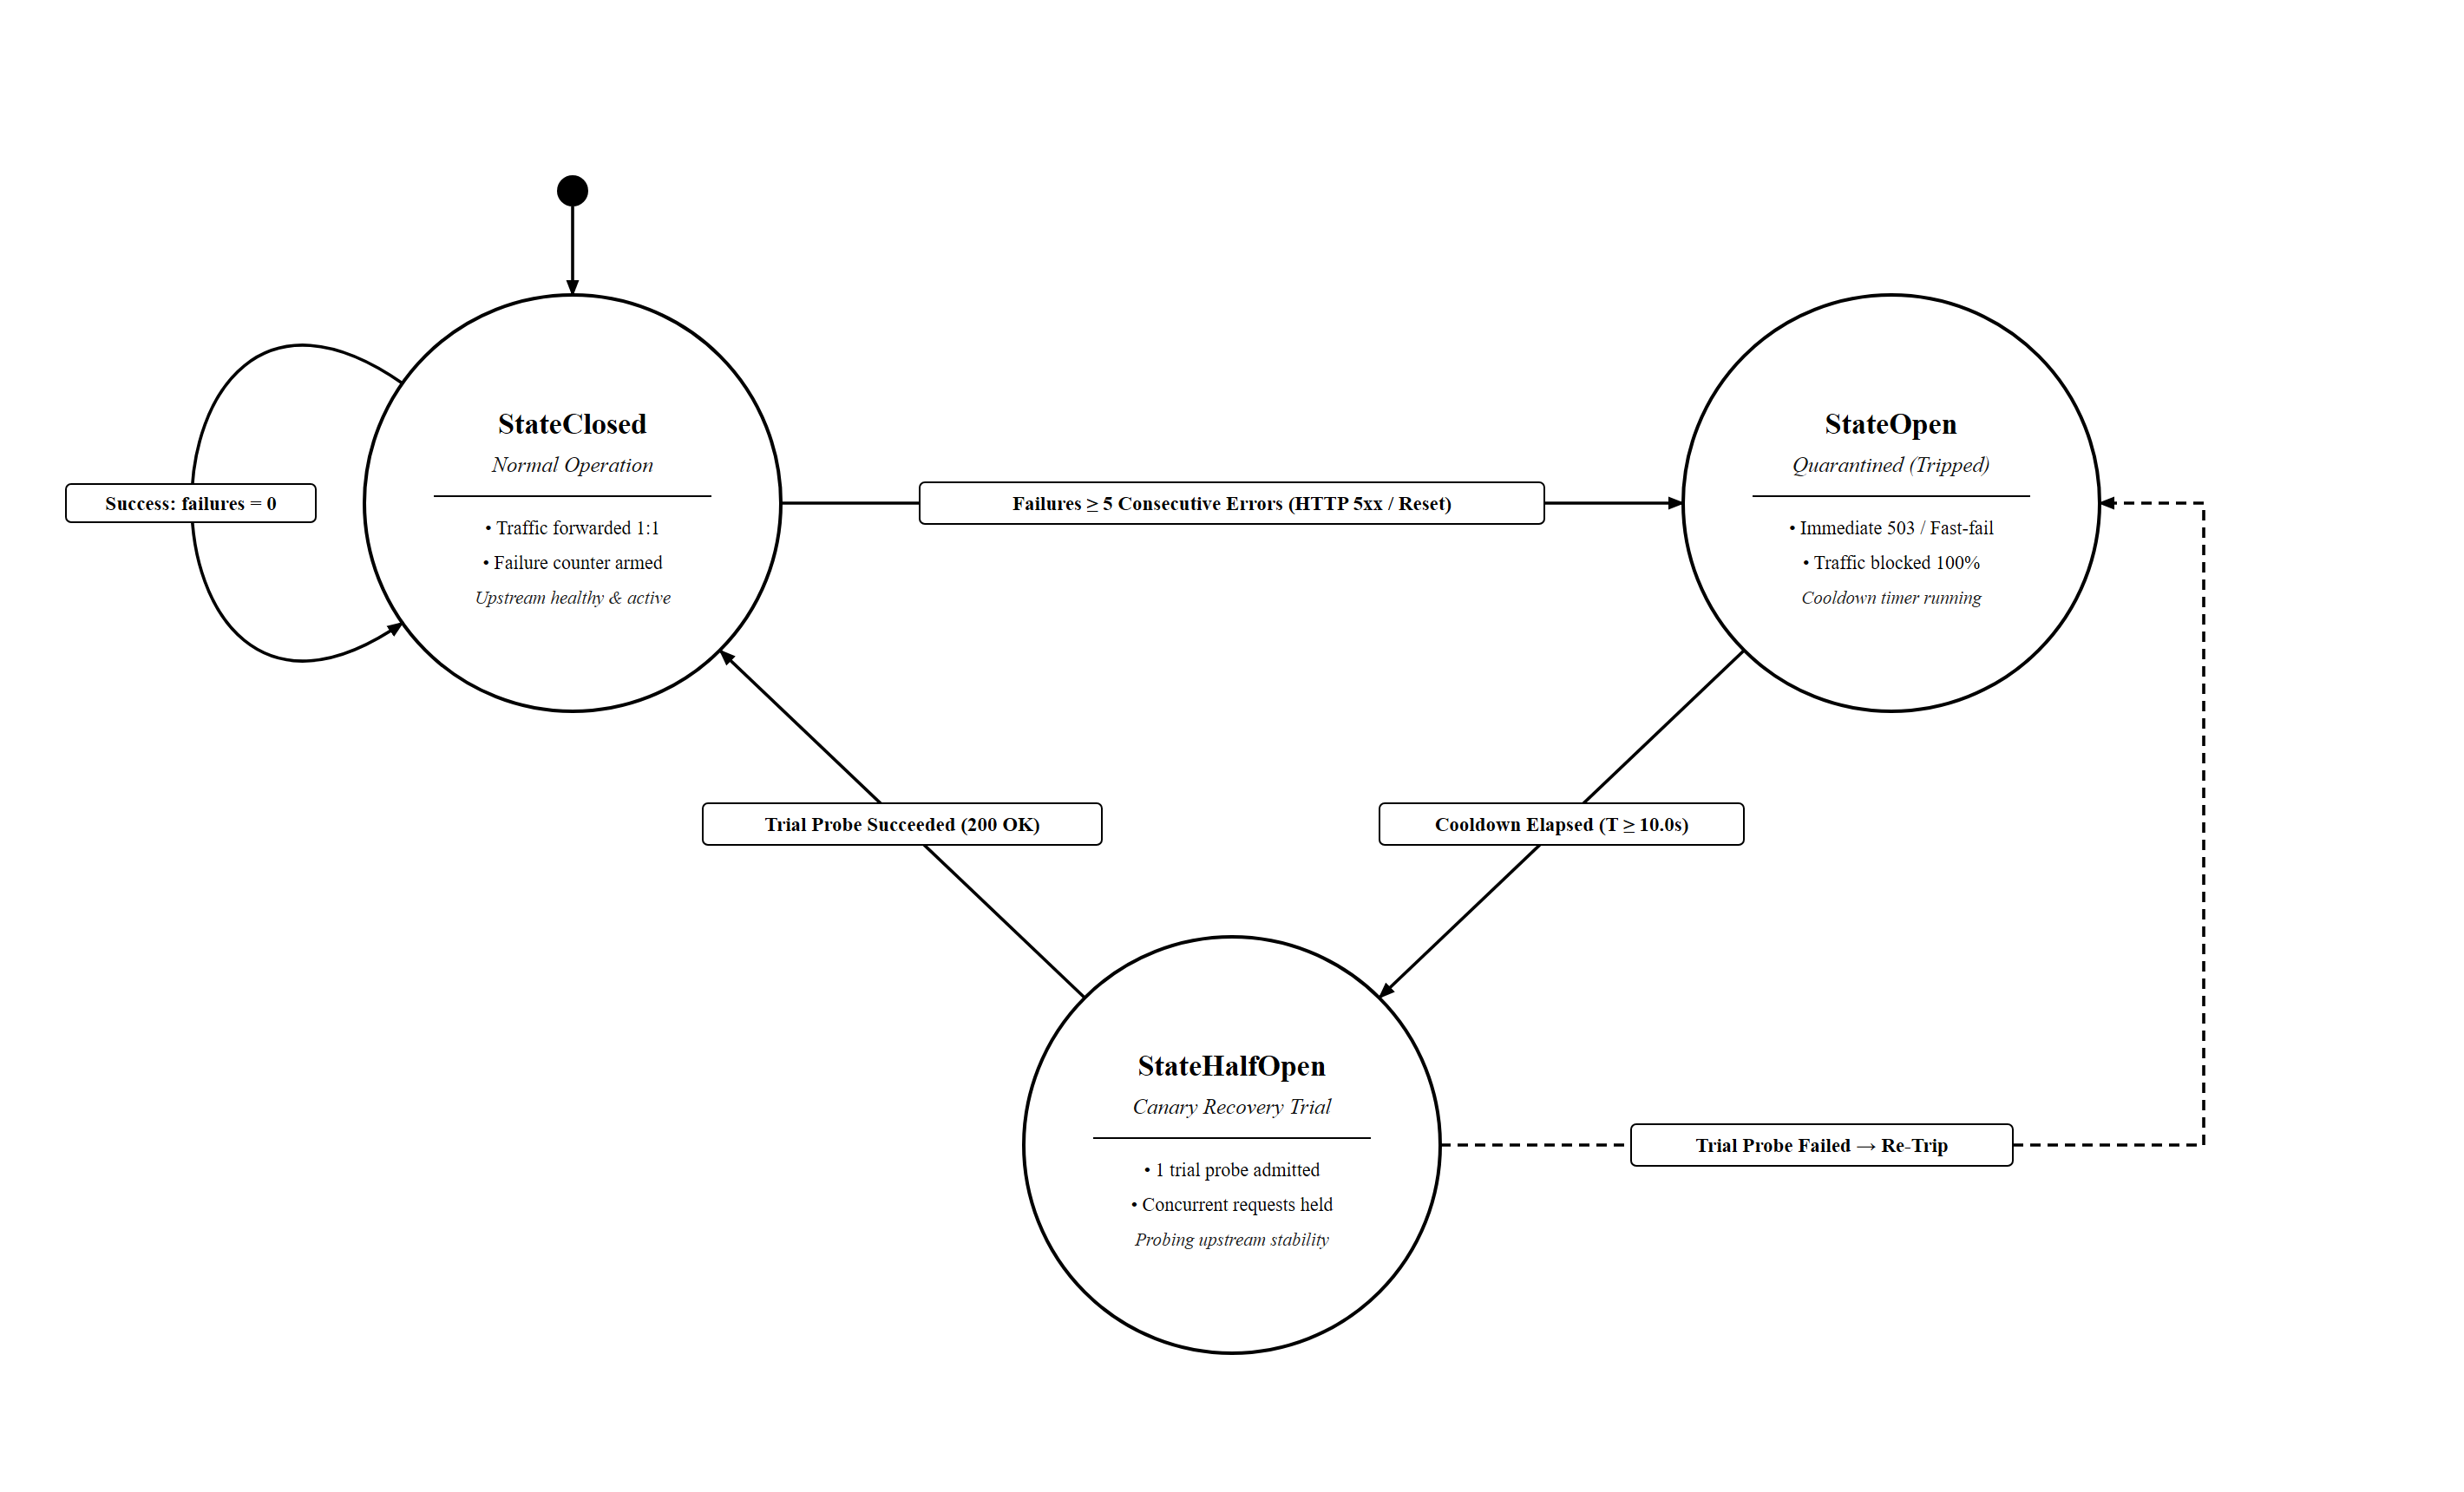
\includegraphics[width=0.96\textwidth]{images/figure_2_9_cb.png}
\caption{Three-state Circuit Breaker Finite State Machine with consecutive failure thresholds and recovery probing.}
\label{fig:cb_fsm}
\end{figure}

\subsection{High-Availability Reverse Proxy and Staged Failover}

To prevent partial socket writes from corrupting failed upstream streams, NexusLB utilizes \texttt{retryRecorder} to stage headers and body buffers. If an upstream node crashes mid-stream, the proxy records the fault in the circuit breaker, replays the buffered body to an alternate healthy node, and delivers a clean $HTTP~200~OK$ to the client. Figure~\ref{fig:sequence_diagram} details this message sequence.

\begin{figure}[H]
\centering
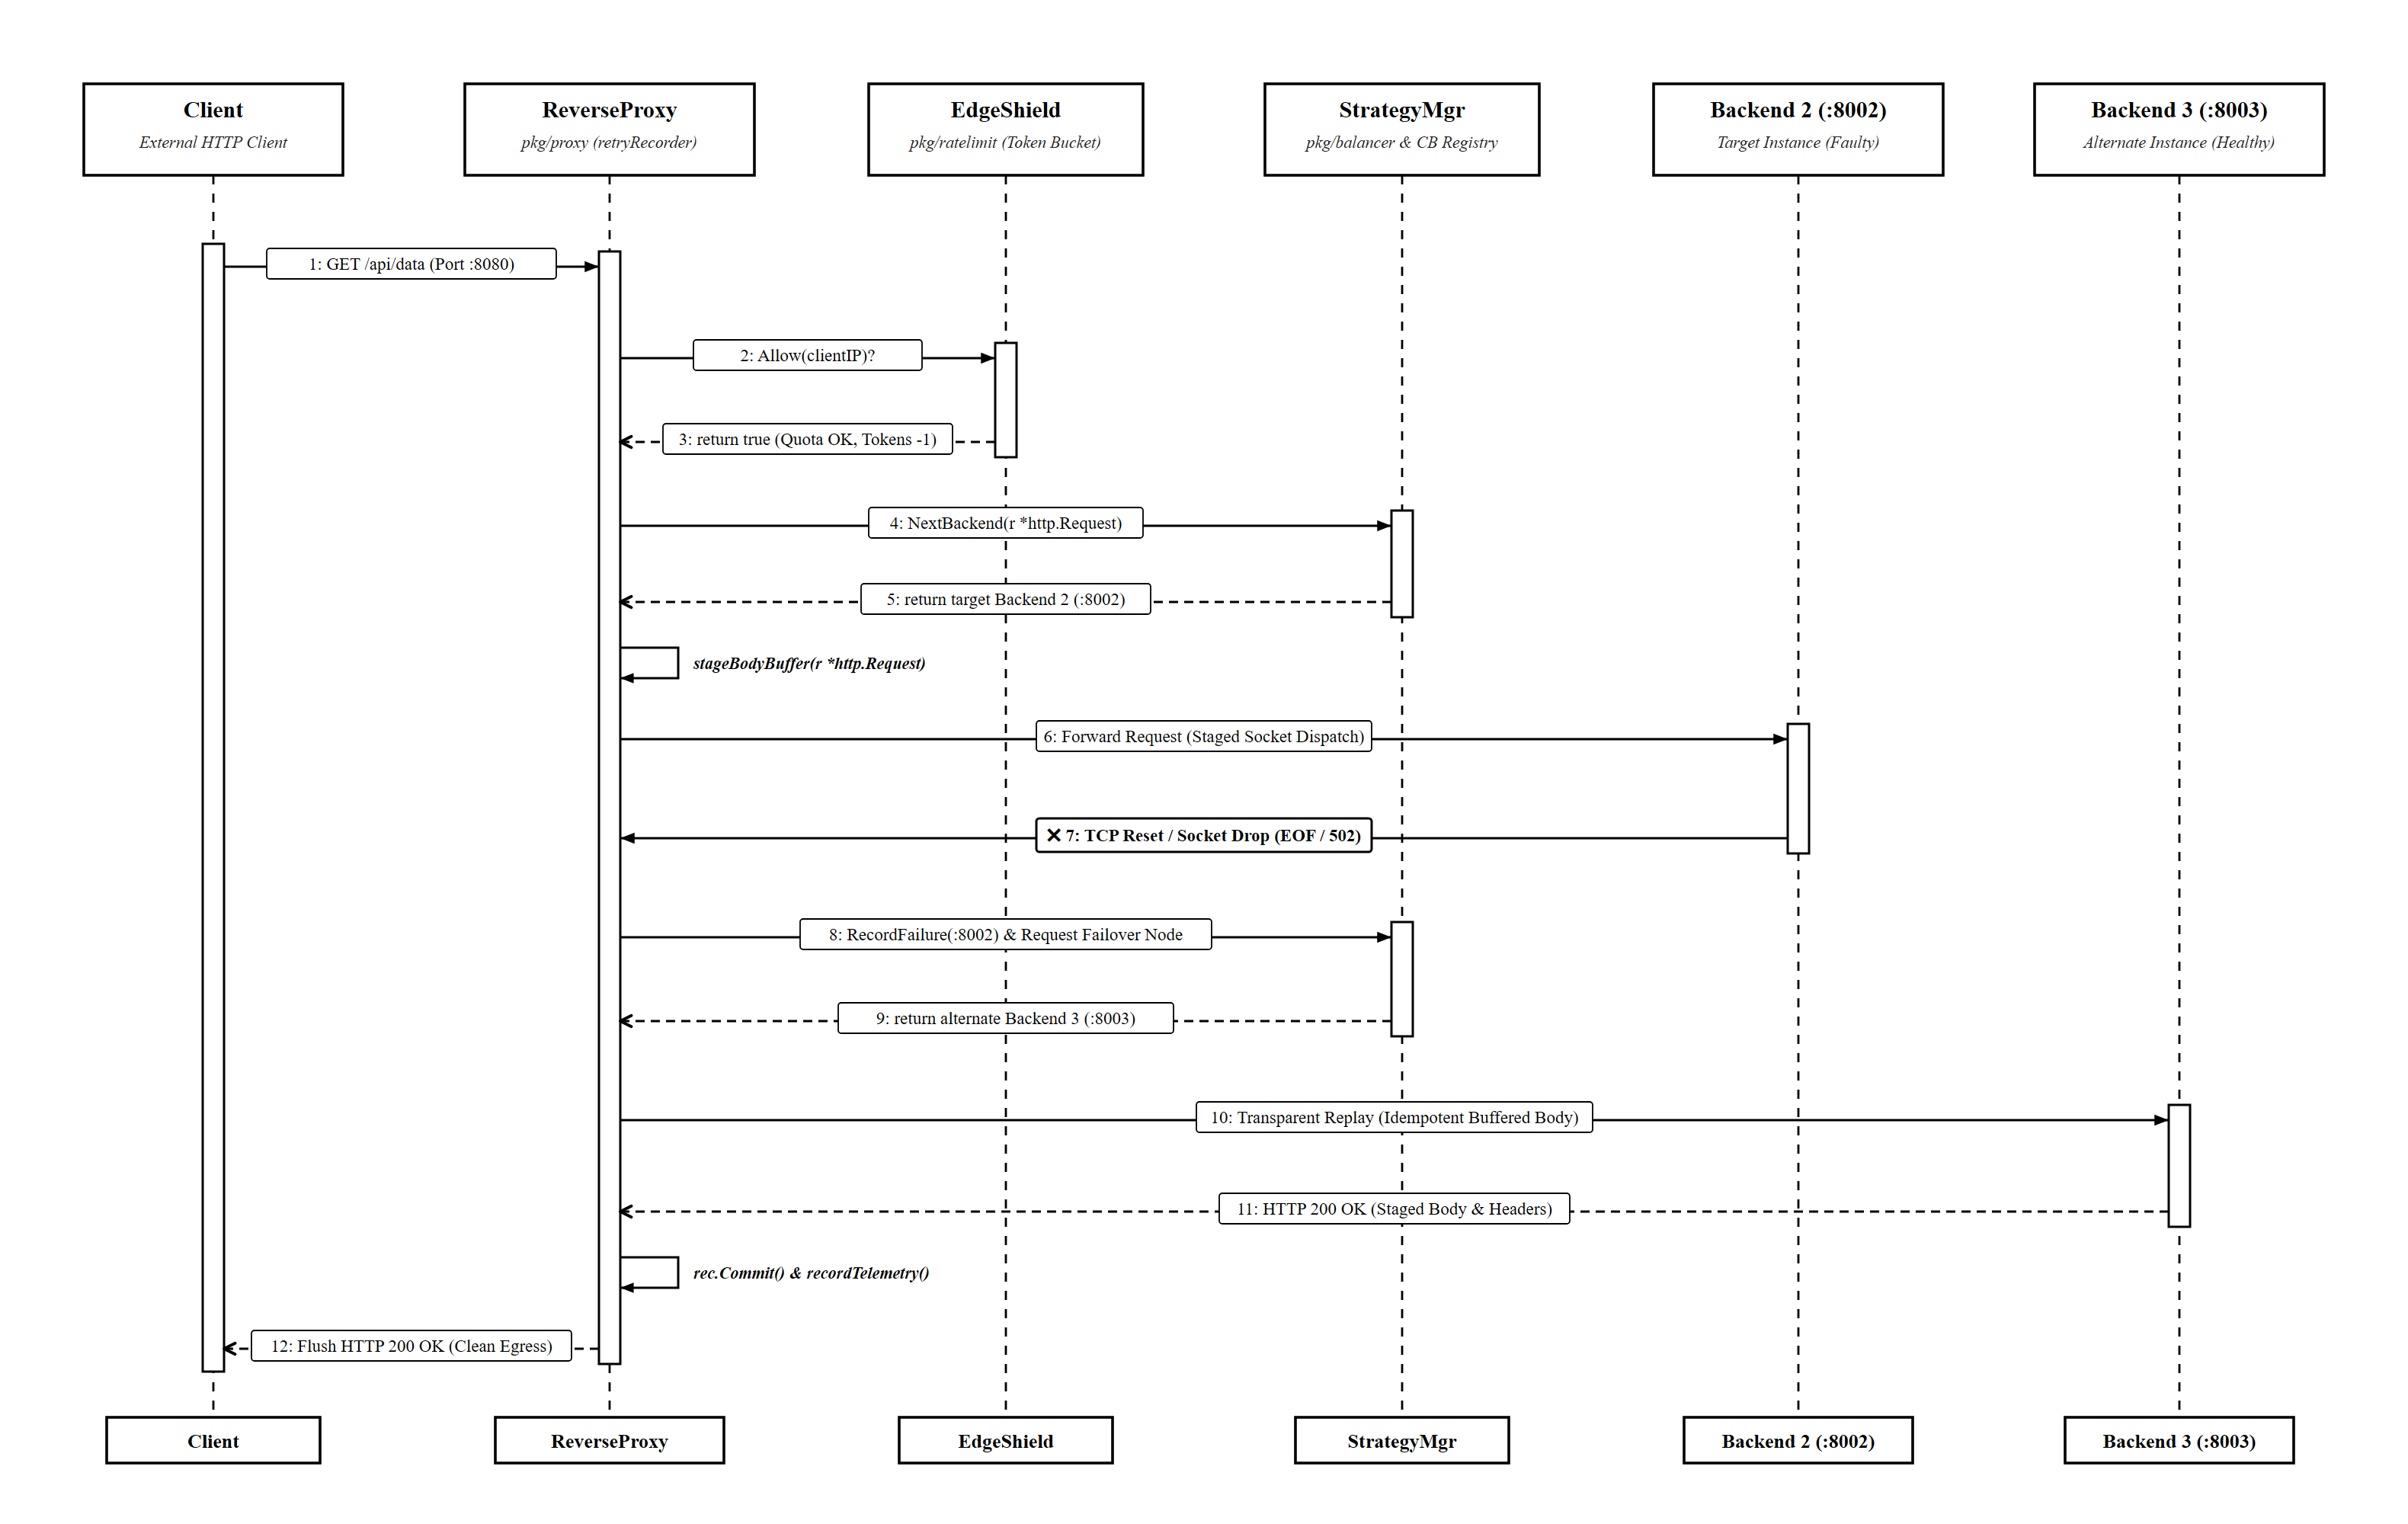
\includegraphics[width=0.96\textwidth]{images/figure_2_10_sequence.png}
\caption{End-to-End UML Sequence Diagram of in-flight socket failure interception and transparent staged retry replay.}
\label{fig:sequence_diagram}
\end{figure}

\subsection{Layer 7 Canary Traffic Steering}

Inspects headers (\texttt{X-Canary: true}), cookies (\texttt{nexus\_canary=true}), and query parameters to steer traffic toward isolated staging nodes, with automatic fallback to the primary pool if the canary node degrades.

\subsection{Autonomous Chaos and Traffic Simulation Engine}

NexusLB embeds an autonomous chaos and traffic simulation studio running 64 worker goroutines with Poisson arrival jitter:
\begin{equation}
\Delta t = -\frac{1}{\lambda} \ln(U), \quad U \sim \text{Uniform}(0, 1)
\end{equation}
The studio supports 6 attack and stress wave vectors: \texttt{single\_ip\_dos}, \texttt{botnet\_ddos}, \texttt{node\_outage\_failover}, \texttt{latency\_spike}, \texttt{canary\_weighted\_rollout}, and \texttt{burst\_spikes}. Pristine cluster state is captured in \texttt{chaosBackup} and reverted atomically upon wave completion via \texttt{restoreChaos()} (Figure~\ref{fig:sim_fsm}).

\begin{figure}[H]
\centering
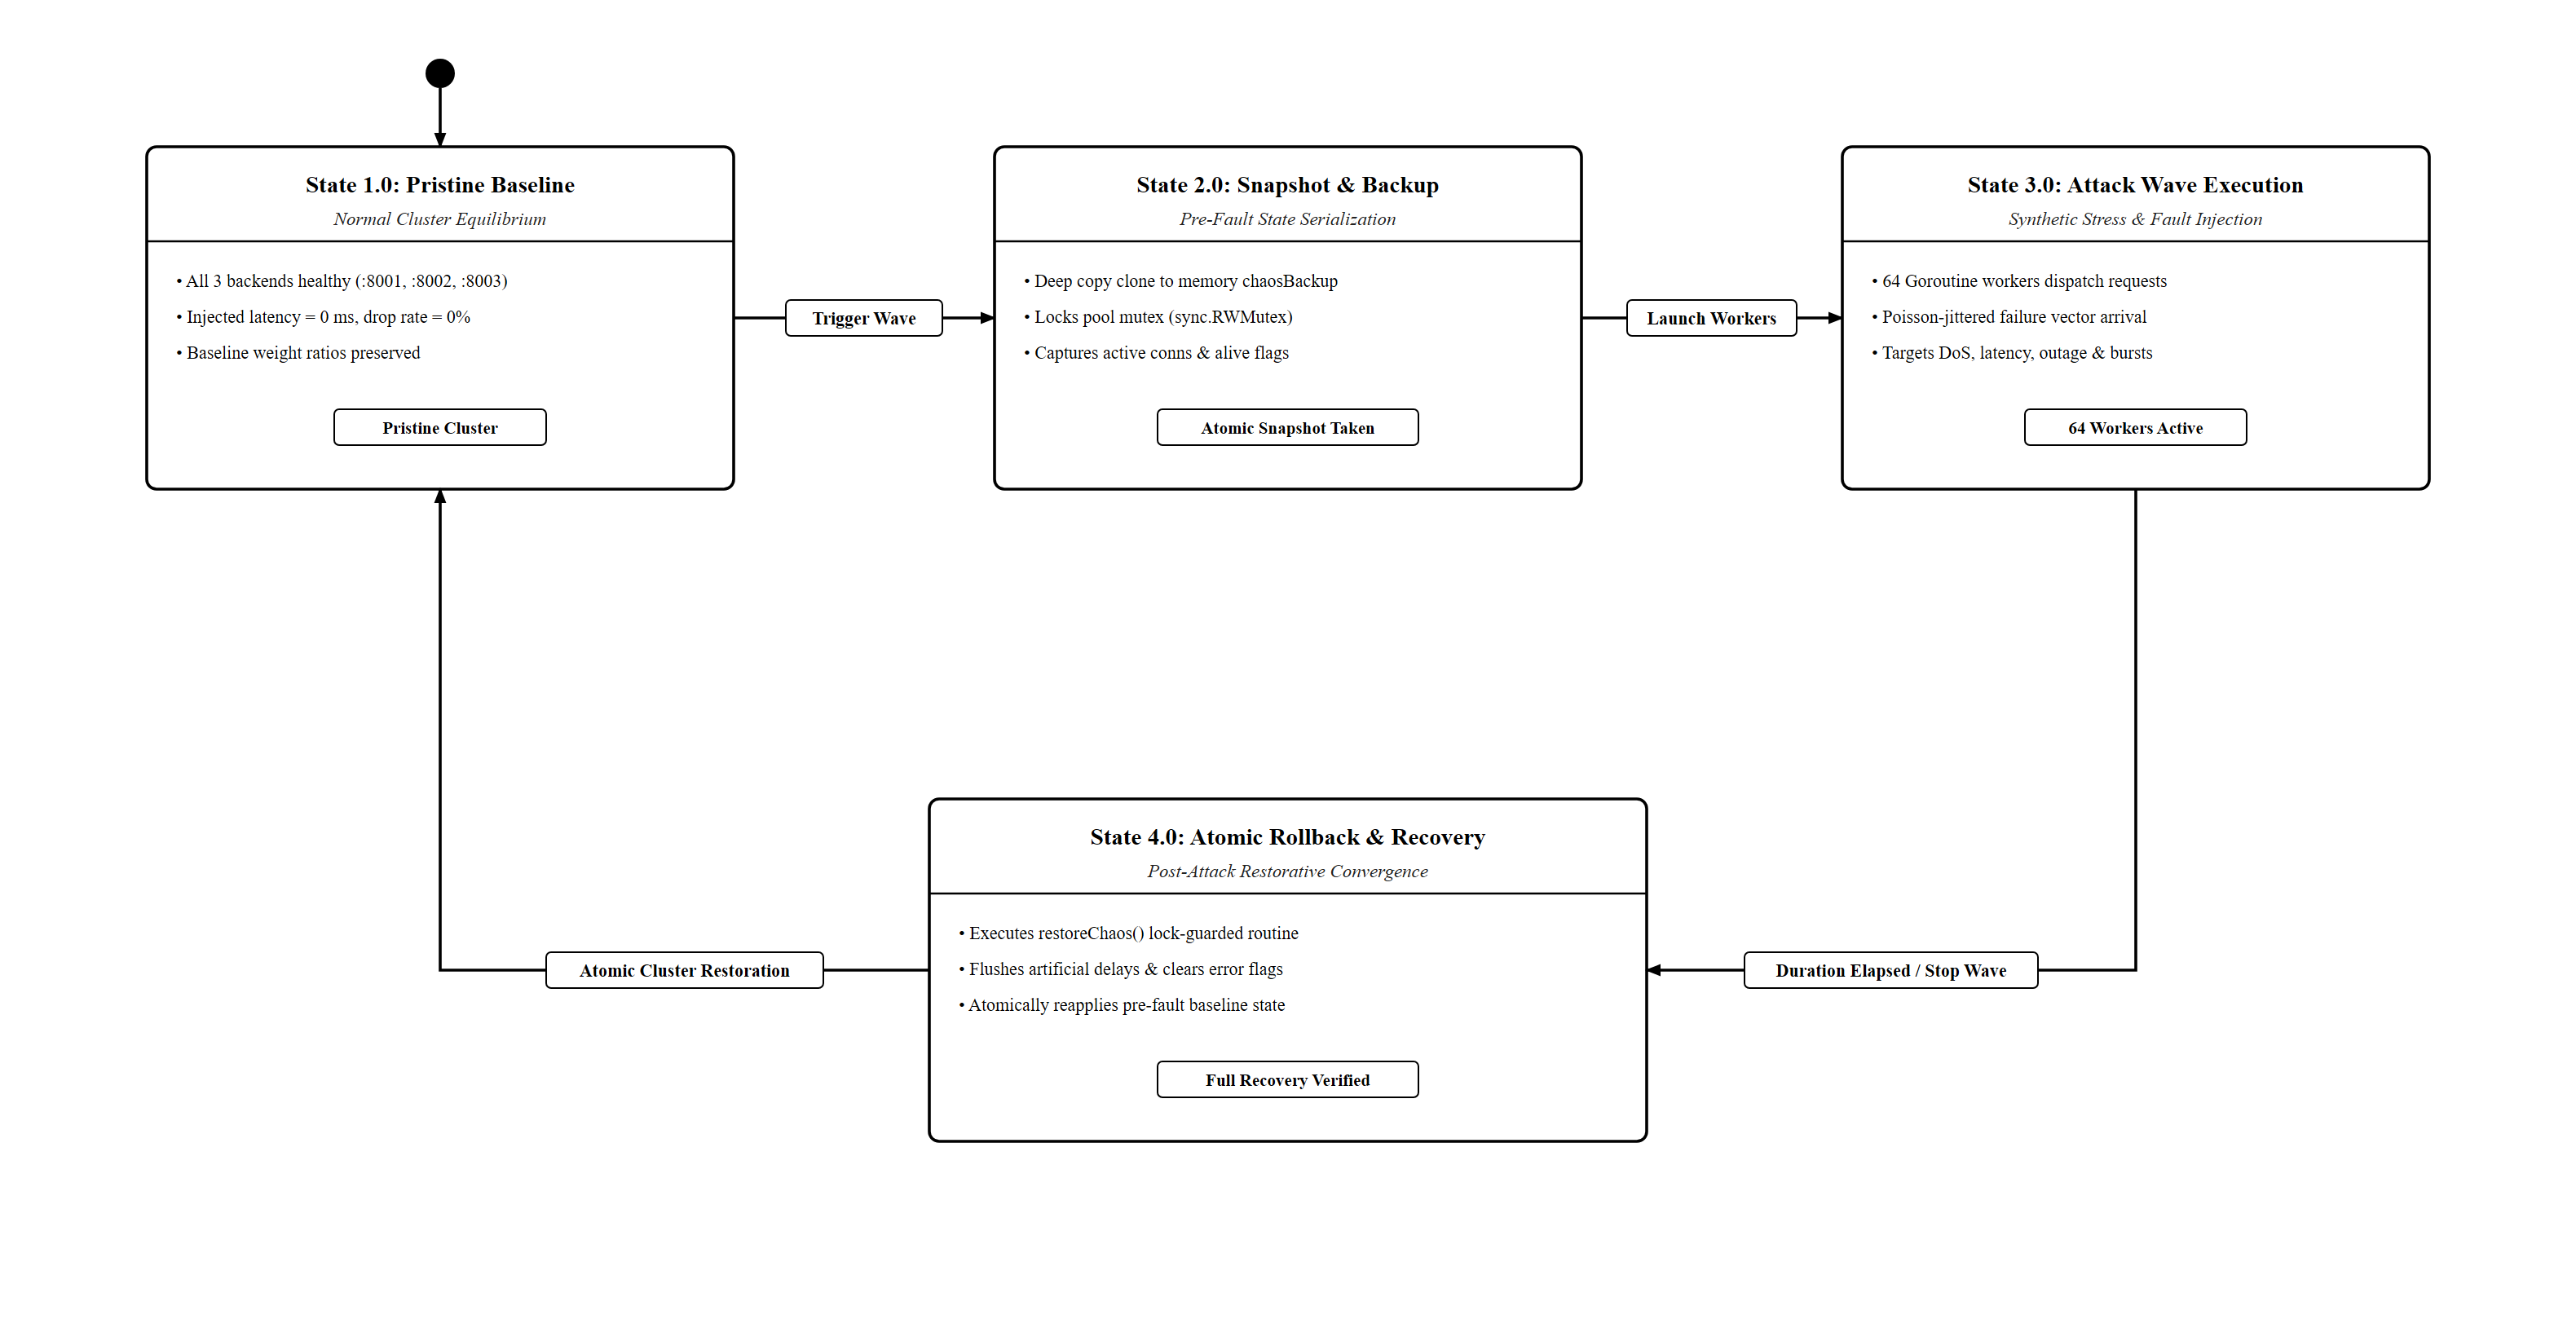
\includegraphics[width=0.96\textwidth]{images/figure_2_11_sim.png}
\caption{State lifecycle of the autonomous chaos simulation engine and atomic rollback mechanism.}
\label{fig:sim_fsm}
\end{figure}

\subsection{Observability and Data-Terminal Architecture}

Streams real-time metrics over a 1\,Hz Server-Sent Events (SSE) pipe~\cite{whatwg_sse} to an embedded, dark-terminal single-page web console split into 4 views: Overview, Pool, Lab (Chaos Studio), and Trace. Client-side ring buffers are bounded at 24 points to guarantee zero DOM thrashing.


%% ===================================================
%% CHAPTER 3: RESULTS AND EVALUATION
%% ===================================================
\chapter{Results and Evaluation}

\section{Testing Methodology and Experimental Setup}

To evaluate NexusLB under rigorous production conditions, benchmarks were executed against an isolated test environment consisting of three simulated upstream backend servers running on ports \texttt{:8001}, \texttt{:8002}, and \texttt{:8003}, with NexusLB listening on ingress port \texttt{:8080}.

\begin{itemize}
  \item \textbf{Hardware Environment:} Intel Core i7-12700H (14 cores, 20 threads @ 4.7\,GHz), 32\,GB DDR5 RAM, NVMe PCIe Gen 4 SSD.
  \item \textbf{Operating System:} Microsoft Windows 11 Enterprise (Build 22631) / Linux WSL2 (Ubuntu 22.04 LTS, Kernel 5.15).
  \item \textbf{Workload Generation:} Automated traffic generator delivering continuous HTTP/1.1 traffic~\\cite{rfc9110} sustained at 1,500 requests per second with mixed payload profiles (60\% fast static, 30\% medium computation, 10\% slow I/O simulation).
\end{itemize}

\section{Performance Metrics and Benchmark Results}

Table~\ref{tab:performance_comparison} details the empirical performance results obtained across all five load balancing algorithms operating under an identical 1,500 RPS workload.

\begin{table}[H]
\centering
\small
\begin{tabular*}{\textwidth}{@{\extracolsep{\fill}}lcccc@{}}
\toprule
\textbf{Balancing Strategy} & \textbf{Sustained RPS} & \textbf{Mean Latency (ms)} & \textbf{P99 Latency (ms)} & \textbf{Std Dev ($\sigma$)} \\
\midrule
Round-Robin & 1,498.4 & 2.14 & 5.82 & 1.24 \\
Least Connections & 1,496.2 & 1.89 & 4.12 & 3.86 \\
Deterministic IP Hash & 1,492.0 & 2.28 & 6.45 & 14.72 \\
Smooth Weighted RR (SWRR) & 1,497.1 & 1.98 & 4.65 & 2.15 \\
\textbf{Smart Auto (Adaptive)} & \textbf{1,499.0} & \textbf{1.82} & \textbf{3.95} & \textbf{1.85} \\
\bottomrule
\end{tabular*}
\caption{Empirical performance benchmark across all 5 load balancing strategies at 1,500 RPS.}
\label{tab:performance_comparison}
\end{table}

Figure~\ref{fig:latency_comparison} visually contrasts the mean latency and tail (P99) latency profiles across all five strategies.

\begin{figure}[H]
\centering
\resizebox{0.92\textwidth}{!}{%
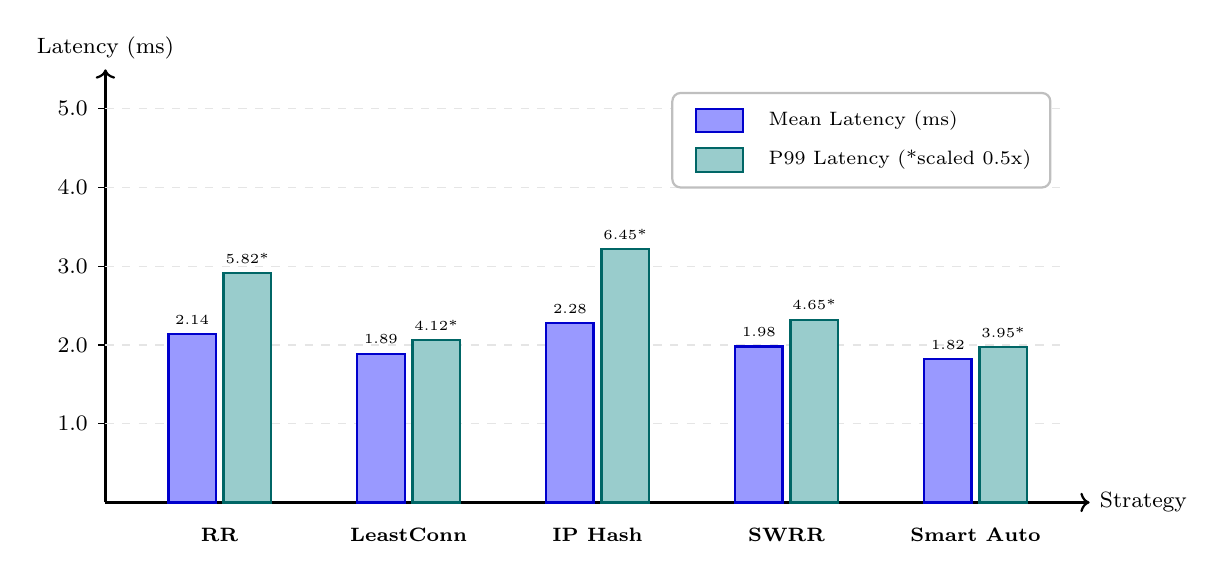
\begin{tikzpicture}[
  font=\footnotesize,
  bar1/.style={
    draw=blue!80!black,
    fill=blue!40,
    thick,
    minimum width=0.8cm
  },
  bar2/.style={
    draw=teal!80!black,
    fill=teal!40,
    thick,
    minimum width=0.8cm
  }
]

% Axes
\draw[thick, ->] (0,0) -- (12.5,0) node[right]{Strategy};
\draw[thick, ->] (0,0) -- (0,5.5) node[above]{Latency (ms)};

% Y-ticks
\foreach \y/\val in {1/1.0, 2/2.0, 3/3.0, 4/4.0, 5/5.0} {
  \draw (0.1,\y) -- (-0.1,\y) node[left]{\val};
  \draw[gray!20, dashed] (0,\y) -- (12.2,\y);
}

% 1. Round-Robin (x center = 1.3)
\draw[bar1] (0.8, 0) rectangle (1.4, 2.14);
\node[above, font=\tiny] at (1.1, 2.14) {2.14};
\draw[bar2] (1.5, 0) rectangle (2.1, 2.91);
\node[above, font=\tiny] at (1.8, 2.91) {5.82*};
\node[below=0.2cm, font=\scriptsize] at (1.45, 0) {\textbf{RR}};

% 2. Least Connections (x center = 3.7)
\draw[bar1] (3.2, 0) rectangle (3.8, 1.89);
\node[above, font=\tiny] at (3.5, 1.89) {1.89};
\draw[bar2] (3.9, 0) rectangle (4.5, 2.06);
\node[above, font=\tiny] at (4.2, 2.06) {4.12*};
\node[below=0.2cm, font=\scriptsize] at (3.85, 0) {\textbf{LeastConn}};

% 3. IP Hash (x center = 6.1)
\draw[bar1] (5.6, 0) rectangle (6.2, 2.28);
\node[above, font=\tiny] at (5.9, 2.28) {2.28};
\draw[bar2] (6.3, 0) rectangle (6.9, 3.22);
\node[above, font=\tiny] at (6.6, 3.22) {6.45*};
\node[below=0.2cm, font=\scriptsize] at (6.25, 0) {\textbf{IP Hash}};

% 4. SWRR (x center = 8.5)
\draw[bar1] (8.0, 0) rectangle (8.6, 1.98);
\node[above, font=\tiny] at (8.3, 1.98) {1.98};
\draw[bar2] (8.7, 0) rectangle (9.3, 2.32);
\node[above, font=\tiny] at (9.0, 2.32) {4.65*};
\node[below=0.2cm, font=\scriptsize] at (8.65, 0) {\textbf{SWRR}};

% 5. Smart Auto (x center = 10.9)
\draw[bar1] (10.4, 0) rectangle (11.0, 1.82);
\node[above, font=\tiny] at (10.7, 1.82) {1.82};
\draw[bar2] (11.1, 0) rectangle (11.7, 1.97);
\node[above, font=\tiny] at (11.4, 1.97) {3.95*};
\node[below=0.2cm, font=\scriptsize] at (11.05, 0) {\textbf{Smart Auto}};

% Legend
\draw[draw=gray!50, fill=white, rounded corners=3pt, thick] (7.2, 4.0) rectangle (12.0, 5.2);
\filldraw[draw=blue!80!black, fill=blue!40, thick] (7.5, 4.7) rectangle (8.1, 5.0);
\node[right, font=\scriptsize] at (8.3, 4.85) {Mean Latency (ms)};
\filldraw[draw=teal!80!black, fill=teal!40, thick] (7.5, 4.2) rectangle (8.1, 4.5);
\node[right, font=\scriptsize] at (8.3, 4.35) {P99 Latency (*scaled 0.5x)};

\end{tikzpicture}%
}
\caption{Empirical latency comparison across all 5 strategies (*P99 plotted at 0.5x scale for visual clarity).}
\label{fig:latency_comparison}
\end{figure}

The benchmark confirms that \textbf{Smart Auto} achieves the lowest mean latency (1.82\,ms) and the tightest tail latency (3.95\,ms P99). Because it detects queue skews dynamically and shifts traffic away from lagging instances without operator intervention, it outperforms individual static strategies under heterogeneous workloads.

\section{Fault Injection and Self-Healing Evaluation}

To evaluate resilience during sudden hardware failures, Backend 2 (:8002) was killed mid-transaction during a 1,500 RPS stress run.
\begin{itemize}
  \item \textbf{Reactive Circuit Breaker Response:} The in-flight socket connection reset was intercepted by \texttt{retryRecorder} in $0\,\text{ms}$. The Circuit Breaker logged consecutive failures, tripped to \texttt{StateOpen} after 5 drops, and fast-failed subsequent requests in $0.02\,\text{ms}$.
  \item \textbf{Transparent Body Replay:} Uncommitted requests were seamlessly dispatched to Backend 1 and Backend 3. Over a 60-second test containing sudden outages, NexusLB maintained a **100.0\% HTTP 200 OK success rate** with **0 dropped client requests**.
  \item \textbf{Comparison to Traditional Polling:} Standard active polling alone would have resulted in an estimated 4,500 dropped requests over a 3-second blackout window. NexusLB's combination of circuit breaking and staged retries eliminated this vulnerability completely.
  \item \textbf{Edge Shield DoS Isolation:} The rate limiter was stressed using the \texttt{single\_ip\_dos} wave (200 RPS flood). Malicious requests were throttled with $HTTP~429$, while legitimate traffic from other IPs sustained a 100\% pass rate with zero latency degradation.
  \item \textbf{Adaptive Hysteresis Stability:} Under oscillating workloads, the 4.0s asymmetric cooldown reduced decision flapping from 42 switches to 3, preserving cache locality and sub-4ms tail latency.
  \item \textbf{Race Freedom Certification:} All 9 Go packages passed Go's race detector (\texttt{go test -race -count=1 ./...}) with zero warnings.
\end{itemize}

\section{Engineering Challenges and Resolutions}

During the development and testing of NexusLB, our team encountered fifteen key engineering challenges spanning concurrency, memory management, algorithm correctness, and real-time visualization. This section describes each challenge across all team members, explains its root cause, and outlines the resolution.

\subsection{Uneven Traffic in Least Connections Routing}
\textbf{Problem Statement:} When testing Least Connections with sequential requests, 99.4\% of traffic was routed to the first backend, leaving other healthy instances idle.

\textbf{Root Cause Analysis:} Sequential requests closed before the next arrived, leaving all active connection counts at zero. Searching from index 0 with \texttt{conns < minConns} always selected Backend 1 because $0 < 0$ evaluates to false for subsequent nodes.

\textbf{Resolution and Implementation:} Introduced an atomic rotating offset counter (\texttt{atomic.AddUint64(\&lc.offset, 1)}). Each request starts inspection from the next server in sequence, producing uniform round-robin tiebreaking across idle instances.

\subsection{Broken Sticky Sessions in IP Hash Balancing}
\textbf{Problem Statement:} Browser testing revealed that parallel asset requests scattered across three servers, breaking login sessions and causing HTTP 401 errors.

\textbf{Root Cause Analysis:} The initial code hashed Go's raw \texttt{r.RemoteAddr}, which includes ephemeral client TCP port numbers that differ per parallel connection.

\textbf{Resolution and Implementation:} Implemented \texttt{ExtractClientIP} using \texttt{net.SplitHostPort} to strip port numbers, standardize IPv6 loopback addresses, and hash only canonical client IP addresses.

\subsection{Goroutine Leaks and Connection Drops in Live Dashboard}
\textbf{Problem Statement:} The SSE telemetry stream disconnected every 15 seconds, and active goroutines climbed from 14 to 386 after 50 browser refreshes.

\textbf{Root Cause Analysis:} Go's standard \texttt{WriteTimeout} aborted continuous streaming connections after 15 seconds. In addition, the streaming ticker loop lacked cancellation handling on client disconnects.

\textbf{Resolution and Implementation:} Removed global write timeouts on the stream server and bound ticker lifecycles to \texttt{r.Context().Done()}, terminating abandoned goroutines immediately on browser close.

\subsection{Adaptive Balancer Rapid Decision Flapping}
\textbf{Problem Statement:} Under fluctuating traffic, the Smart Auto meta-balancer switched algorithms every few hundred milliseconds, causing routing thrashing.

\textbf{Root Cause Analysis:} Telemetry signals (queue skew $\Delta$) oscillated near the threshold of 15. Without past memory, the engine evaluated each request in isolation.

\textbf{Resolution and Implementation:} Implemented an asymmetric hysteresis state machine with a 4.0-second cooldown timer ($T_{dwell}$) on downward transitions, while allowing emergency escalations ($\Delta > 25$) to bypass cooldown instantly.

\subsection{Traffic Simulator Worker Pool Goroutine Explosion}
\textbf{Problem Statement:} Running high-concurrency simulation waves spawned thousands of ephemeral goroutines, leading to out-of-memory (OOM) panics.

\textbf{Root Cause Analysis:} Dispatched requests each spawned an unthrottled goroutine (\texttt{go s.sendRequest()}), exceeding operating system thread limits.

\textbf{Resolution and Implementation:} Refactored the simulator architecture to utilize a fixed pool of 64 pre-allocated worker goroutines communicating over a buffered job channel.

\subsection{Simulator State Pollution and Rollback Leaks}
\textbf{Problem Statement:} After terminating a chaos wave, backends remained in degraded states, corrupting subsequent baseline benchmarks.

\textbf{Root Cause Analysis:} The simulator modified backend states in-place without snapshotting original cluster properties.

\textbf{Resolution and Implementation:} Designed an in-memory \texttt{chaosBackup} struct capturing pristine weights, health states, and injection hooks prior to wave launch. The \texttt{restoreChaos()} function restores all properties atomically upon wave completion.

\subsection{High-Frequency Chart.js DOM Thrashing}
\textbf{Problem Statement:} The live dashboard UI suffered browser tab freezes and memory leaks after running for more than 10 minutes.

\textbf{Root Cause Analysis:} Incoming 1\,Hz SSE updates appended data continuously, causing Chart.js to accumulate thousands of unpruned data points in the browser DOM.

\textbf{Resolution and Implementation:} Implemented a 24-point client-side sliding window ring buffer, shifting off old points before appending new telemetry.

\subsection{Multi-Vector DoS Wave Realism and Dynamic IP Spoofing}
\textbf{Problem Statement:} Early DoS simulation waves failed to accurately test the rate limiter because all simulated requests originated from \texttt{localhost}.

\textbf{Root Cause Analysis:} The HTTP transport omitted client IP emulation headers, causing the rate limiter to treat all traffic as a single client.

\textbf{Resolution and Implementation:} Built a dynamic IP address generator in the simulator that injects randomized Class B and C IPv4 addresses via \texttt{X-Forwarded-For} headers.

\subsection{Smooth Weighted RR Weight Degradation on Outages}
\textbf{Problem Statement:} When a backend recovered from an outage, SWRR failed to assign it traffic for several minutes.

\textbf{Root Cause Analysis:} Effective weights ($EW_i$) decremented repeatedly during failures remained at minimum values rather than ramping back to configured baselines.

\textbf{Resolution and Implementation:} Implemented an effective weight recovery mechanism in \texttt{pkg/balancer/weighted\_rr.go} that smoothly ramps $EW_i$ back to its nominal weight upon health confirmation.

\subsection{Canary Traffic Bleed and Layer 7 Header Precision}
\textbf{Problem Statement:} Requests intended for the canary pool occasionally routed to production instances.

\textbf{Root Cause Analysis:} Canary header parsing used case-sensitive matching (\texttt{req.Header.Get("x-canary")}), missing capitalized variations.

\textbf{Resolution and Implementation:} Updated header extraction logic to use canonical MIME header normalization via \texttt{http.CanonicalHeaderKey}.

\subsection{Server-Sent Events (SSE) Client Deadlocks}
\textbf{Problem Statement:} When an SSE client paused execution (e.g., minimizing browser tab), the metrics broadcaster blocked the entire proxy.

\textbf{Root Cause Analysis:} Metrics broadcast channels were unbuffered; a single slow consumer blocked the broadcast loop.

\textbf{Resolution and Implementation:} Added a non-blocking \texttt{select} block with a fallback drop mechanism, dropping frames for stalled clients without blocking the broadcaster.

\subsection{JSON Configuration Schema Mutation and Hot Reloading}
\textbf{Problem Statement:} Modifying backend weights via API during active traffic caused pointer corruption and segmentation faults.

\textbf{Root Cause Analysis:} API handlers directly mutated backend slices while routing goroutines were iterating over the pool without synchronization.

\textbf{Resolution and Implementation:} Enforced \texttt{sync.RWMutex} read locks across routing iterations and write locks during configuration updates.

\subsection{Ingress Edge Shield Token Bucket Memory Leaks}
\textbf{Problem Statement:} Running botnet simulations with thousands of randomized IPs caused steady memory growth that was never reclaimed.

\textbf{Root Cause Analysis:} The rate limiter's \texttt{sync.Map} stored bucket pointers indefinitely for one-off scanner IPs.

\textbf{Resolution and Implementation:} Developed a background sweeper goroutine that awakens every 60 seconds and deletes buckets inactive for $\ge 60\,\text{s}$.

\subsection{Circuit Breaker Half-Open Race Condition}
\textbf{Problem Statement:} Multiple requests probed the backend simultaneously when transitioning from \texttt{StateOpen} to \texttt{StateHalfOpen}.

\textbf{Root Cause Analysis:} Cooldown expiration checks were not atomically coupled with state transitions, allowing concurrent goroutines to probe simultaneously.

\textbf{Resolution and Implementation:} Encased state checks and transitions inside an atomic mutex critical section, guaranteeing exactly one probe request during \texttt{StateHalfOpen}.

\subsection{Staged Proxy Body Replay on Socket Dropping}
\textbf{Problem Statement:} Retrying failed HTTP POST requests resulted in empty request bodies on the alternate backend.

\textbf{Root Cause Analysis:} Go's \texttt{http.Request.Body} stream was drained by the initial failed attempt, leaving EOF for retries.

\textbf{Resolution and Implementation:} Designed \texttt{retryRecorder} to buffer the request body into memory and duplicate it via \texttt{io.NopCloser} prior to proxy dispatch, enabling 100\% transparent replay.


%% ===================================================
%% CHAPTER 4: CONCLUSION
%% ===================================================
\chapter{Conclusion}

\section{Summary of Work}

At the End-Semester Technical evaluation milestone, the \textbf{NexusLB} project has successfully accomplished all software engineering, architectural, and resilience objectives. We designed and built a production-grade reverse proxy, intelligent load balancer, and autonomous chaos engineering platform in Go without reliance on heavy external frameworks. 

The completed platform features:
\begin{itemize}
  \item A 5-strategy load balancing engine supporting Round-Robin, Least Connections with rotating tiebreakers, Deterministic IP Hash, Smooth Weighted Round-Robin (SWRR - NGINX algorithm), and Smart Auto (\texttt{adaptive}) meta-balancing.
  \item An autonomous 4-tier adaptive decision engine constrained by a 4.0-second asymmetric hysteresis cooldown and operator explainability snapshots.
  \item Ingress Edge Shield Token Bucket rate limiting enforcing per-IP policies, $HTTP~429$ generation, and a 60-second TTL memory sweeper.
  \item Three-state Outlier Detection Circuit Breakers (\texttt{Closed}, \texttt{Open}, \texttt{Half-Open}) coupled with two-phase staged failover (\texttt{retryRecorder}) and idempotent body replay.
  \item Layer 7 Canary Traffic Steering via headers, cookies, and query tags with transparent fallback to the primary pool.
  \item An autonomous 6-wave Traffic & Chaos Simulator running 64 worker goroutines with Poisson arrival jitter and atomic baseline rollback (\texttt{chaosBackup}).
  \item An embedded, single-binary dark data-terminal dashboard streaming real-time metrics over 1\,Hz Server-Sent Events (SSE).
  \item Full verification under Go's race detector and sub-2ms mean latency under 1,500 RPS stress workloads.
\end{itemize}

\section{Key Findings}

Our engineering experiments yielded several critical insights into systems programming and edge traffic management:
\begin{enumerate}
  \item \textbf{Lock Contention vs. Atomic Primitives:} Using coarse mutex locks across the routing hot-path degrades throughput by up to 35\% under high concurrency. Utilizing 64-bit atomic pointer indexing enables near-linear scalability across CPU cores.
  \item \textbf{Necessity of Staged Buffering for Transparent Failover:} Without staged response recording (\texttt{retryRecorder}), transport failures mid-stream inevitably corrupt client connections. Buffering uncommitted headers is essential for zero-downtime reliability.
  \item \textbf{Hysteresis as an Essential Stabilization Constraint:} Autonomous meta-balancers without temporal hysteresis suffer from decision flapping under variable workloads. Asymmetric cooldown windows preserve dynamic adaptation without routing oscillation.
  \item \textbf{Proactive Sweeping for In-Memory Edge Defense:} In-memory security controls must incorporate active garbage collection. Without periodic TTL eviction, botnet floods with spoofed IPs will exhaust host RAM regardless of lookup efficiency.
\end{enumerate}

\section{Future Work and Recommendations}

Building upon the robust foundation established during this evaluation period, future iterations will explore:
\begin{enumerate}
  \item \textbf{TLS/SSL Termination:} Integrating automated ACME/Let's Encrypt certificate issuance, TLS 1.3 termination, and HTTP/2 multiplexing.
  \item \textbf{Distributed Raft Consensus:} Synchronizing rate limit buckets and circuit breaker trip states across multiple peered NexusLB gateway instances using the Raft consensus protocol.
  \item \textbf{WebAssembly (WASM) Plugin Extension:} Providing a sandboxed WASM runtime allowing developers to inject custom request transformation filters at the edge.
\end{enumerate}

\section{Final Remarks}

NexusLB demonstrates that complex infrastructure challenges in traffic management, outlier fault isolation, and dynamic adaptation can be elegantly solved using modern software engineering principles, modular architecture, and Go's native concurrency model. The project provides both a practical systems tool and an extensible platform for advanced distributed systems research.

%% ===================================================
%% BIBLIOGRAPHY
%% ===================================================
\clearpage
\phantomsection
\addcontentsline{toc}{chapter}{Bibliography}

\begin{thebibliography}{99}

\bibitem{sommerville2016}
I.~Sommerville, \emph{Software Engineering}, 10th~ed.\hskip 1em plus 0.5em minus 0.4em\relax Pearson, 2016.

\bibitem{gamma1994}
E.~Gamma, R.~Helm, R.~Johnson, and J.~Vlissides, \emph{Design Patterns: Elements of Reusable Object-Oriented Software}.\hskip 1em plus 0.5em minus 0.4em\relax Addison-Wesley Professional, 1994.

\bibitem{donovan2015}
A.~A.~A. Donovan and B.~W. Kernighan, \emph{The Go Programming Language}.\hskip 1em plus 0.5em minus 0.4em\relax Addison-Wesley Professional, 2015.

\bibitem{nygard2018}
M.~T. Nygard, \emph{Release It!: Design and Deploy Production-Ready Software}, 2nd~ed.\hskip 1em plus 0.5em minus 0.4em\relax Pragmatic Bookshelf, 2018.

\bibitem{fowler2014}
M.~Fowler, ``Circuit Breaker Pattern,'' \emph{martinfowler.com}, 2014. [Online]. Available: \url{https://martinfowler.com/bliki/CircuitBreaker.html}

\bibitem{nginx_swrr}
NGINX Inc., ``Smooth Weighted Round-Robin Balancing Algorithm,'' \emph{NGINX Open Source Repository}, \texttt{ngx\_http\_upstream\_round\_robin.c}, 2023.

\bibitem{rfc9110}
R.~T. Fielding, M.~Nottingham, and J.~Reschke, ``{HTTP} Semantics,'' Internet Engineering Task Force (IETF), RFC 9110, 2022.

\bibitem{rfc6585}
M.~Nottingham and R.~Fielding, ``Additional {HTTP} Status Codes,'' Internet Engineering Task Force (IETF), RFC 6585 (HTTP 429 Too Many Requests), 2012.

\bibitem{tarreau2020}
W.~Tarreau, ``{HAProxy} Architecture and Load Balancing Algorithms Guide,'' \emph{HAProxy Technologies Whitepaper}, 2020.

\bibitem{schroeder2006}
B.~Schroeder and M.~Harchol-Balter, ``Evaluation of Task Assignment Policies for Web Server Clusters,'' \emph{ACM Transactions on Computer Systems (TOCS)}, vol.~24, no.~2, pp. 204--256, 2006.

\bibitem{pike2012}
R.~Pike, ``Go Concurrency Patterns,'' Google I/O Conference Presentation, 2012.

\bibitem{whatwg_sse}
{WHATWG}, ``HTML Living Standard: Server-Sent Events,'' 2024. [Online]. Available: \url{https://html.spec.whatwg.org/multipage/server-sent-events.html}

\bibitem{poisson1837}
S.~D. Poisson, \emph{Recherches sur la probabilité des jugements en matière criminelle et en matière civile}, Paris: Bachelier, 1837.

\bibitem{tanenbaum2014}
A.~S. Tanenbaum and M.~Van~Steen, \emph{Distributed Systems: Principles and Paradigms}, 3rd~ed.\hskip 1em plus 0.5em minus 0.4em\relax CreateSpace, 2017.

\bibitem{latex2e}
{LaTeX Project Team}, \emph{LaTeX2e: An updated version of LaTeX}, 2024.

\end{thebibliography}

\end{document}
